%\pdfoutput=1
% Uncomment line above if submitting to arXiv and using pdflatex
 
% $Id: main.tex 33041 2013-03-25 16:12:53Z tgershon $
% ============================================================================
% Purpose: Template for LHCb documents
% Authors: Tomasz Skwarnicki, Roger Forty, Ulrik Egede
% Created on: 2010-09-24
% ============================================================================
\documentclass[12pt,a4paper]{article}
% For two column text, add "twocolumn" as an option to the document
% class. Also uncomment the two "onecolumn" and "twocolumn" lines
% around the title page below.
 
% Variables that controls behaviour
\usepackage{ifthen} % for conditional statements
\newboolean{pdflatex}
\setboolean{pdflatex}{true} % False for eps figures
 
\newboolean{articletitles}
\setboolean{articletitles}{true} % False removes titles in references
 
\newboolean{uprightparticles}
\setboolean{uprightparticles}{false} %True for upright particle symbols
 
\newboolean{inbibliography}
\setboolean{inbibliography}{false} %True once you enter the bibliography
 
% THis file contains all the default packages and modifications for
% LHCb formatting

%% %%%%%%%%%%%%%%%%%%
%%  Page formatting
%% %%%%%%%%%%%%%%%%%%
\textheight=230mm
\textwidth=160mm
\oddsidemargin=7mm
\evensidemargin=-10mm
\topmargin=-10mm
\headsep=20mm
\columnsep=5mm
\addtolength{\belowcaptionskip}{0.5em}

\renewcommand{\textfraction}{0.01}
\renewcommand{\floatpagefraction}{0.99}
\renewcommand{\topfraction}{0.9}
\renewcommand{\bottomfraction}{0.9}


\setlength{\hoffset}{-2cm}
\setlength{\voffset}{-2cm}
% Page defaults ...
\topmargin=0.5cm
\oddsidemargin=2.5cm
\textwidth=16cm
\textheight=22cm
% Allow the page size to vary a bit ...
\raggedbottom
% To avoid Latex to be too fussy with line breaking ...
\sloppy

%% %%%%%%%%%%%%%%%%%%%%%%%
%% Packages to be used
%% %%%%%%%%%%%%%%%%%%%%%%% 
\usepackage{microtype}
\usepackage{lineno}  % for line numbering during review
\usepackage{xspace}  % To avoid problems with missing or double spaces after
                     % predefined symbold

%\usepackage{caption}                                      % these three commands get the figure

\usepackage[font=small,justification=RaggedRight]{caption} % these three
\renewcommand{\captionfont}{\small}                        % commands get the
\renewcommand{\captionlabelfont}{\small}                   % figure and table
                                                           % captions
                                                           % automatically small

%% Graphics
\usepackage{graphicx}  % to include figures (can also use other packages)
\usepackage{color}
\usepackage{colortbl}
\graphicspath{{./figs/}} % Make Latex search fig subdir for figures

%% Math
\usepackage{amsmath} % Adds a large collection of math symbols
\usepackage{amssymb}
\usepackage{amsfonts}
\usepackage{upgreek} % Adds in support for greek letters in roman typeset

%% fix to allow peaceful coexistence of line numbering and
%% mathematical objects
%% http://www.latex-community.org/forum/viewtopic.php?f=5&t=163
%%
\newcommand*\patchAmsMathEnvironmentForLineno[1]{%
\expandafter\let\csname old#1\expandafter\endcsname\csname #1\endcsname
\expandafter\let\csname oldend#1\expandafter\endcsname\csname
end#1\endcsname
 \renewenvironment{#1}%
   {\linenomath\csname old#1\endcsname}%
   {\csname oldend#1\endcsname\endlinenomath}%
}
\newcommand*\patchBothAmsMathEnvironmentsForLineno[1]{%
  \patchAmsMathEnvironmentForLineno{#1}%
  \patchAmsMathEnvironmentForLineno{#1*}%
}
\AtBeginDocument{%
\patchBothAmsMathEnvironmentsForLineno{equation}%
\patchBothAmsMathEnvironmentsForLineno{align}%
\patchBothAmsMathEnvironmentsForLineno{flalign}%
\patchBothAmsMathEnvironmentsForLineno{alignat}%
\patchBothAmsMathEnvironmentsForLineno{gather}%
\patchBothAmsMathEnvironmentsForLineno{multline}%
}

% Get hyperlinks to captions and in references.
% These do not work with revtex. Use "hypertext" as class option instead.
\usepackage{hyperref}    % Hyperlinks in references
\usepackage[all]{hypcap} % Internal hyperlinks to floats.

%%% $Id: lhcb-symbols-def.tex 16562 2012-03-01 08:41:50Z uegede $
%%% ======================================================================
%%% Purpose: standard LHCb aliases
%%% Author: Originally Ulrik Egede, adapted by Tomasz Skwarnicki for templates,
%%% rewritten by Chris Parkes
%%% Created on: 2009-09-24
%%% =======================================================================

%%% this has to go before \begin{document}
%%%\usepackage{ifthen} 
%%%\newboolean{uprightparticles}
%%%\setboolean{uprightparticles}{true} %Set to false to get italic particle symbols

%%% Add comments with at least three %%% preceding.
%%% Add new sections with one % preceding
%%% Add new subsections with two %% preceding

%%%%%%%%%%%%%
% Experiments
%%%%%%%%%%%%%
\def\lhcb {LHCb\xspace}
\def\lal {LAL\xspace}
\def\ux85 {UX85\xspace}
\def\cern {CERN\xspace}
\def\lhc {LHC\xspace}
\def\atlas {ATLAS\xspace}
\def\cms {CMS\xspace}
\def\babar  {BaBar\xspace}
\def\belle  {Belle\xspace}
\def\aleph  {ALEPH\xspace}
\def\delphi {DELPHI\xspace}
\def\opal   {OPAL\xspace}
\def\lthree {L3\xspace}
\def\lep    {LEP\xspace}
\def\cdf    {CDF\xspace}
\def\dzero  {D\O\xspace}
\def\sld    {SLD\xspace}
\def\cleo   {CLEO\xspace}
\def\uaone  {UA1\xspace}
\def\uatwo  {UA2\xspace}
\def\tevatron {TEVATRON\xspace}

%% LHCb sub-detectors and sub-systems

\def\pu     {PU\xspace}
\def\velo   {VELO\xspace}
\def\rich   {RICH\xspace}
\def\richone {RICH1\xspace}
\def\richtwo {RICH2\xspace}
\def\ttracker {TT\xspace}
\def\intr   {IT\xspace}
\def\st     {ST\xspace}
\def\ot     {OT\xspace}
\def\Tone   {T1\xspace}
\def\Ttwo   {T2\xspace}
\def\Tthree {T3\xspace}
\def\Mone   {M1\xspace}
\def\Mtwo   {M2\xspace}
\def\Mthree {M3\xspace}
\def\Mfour  {M4\xspace}
\def\Mfive  {M5\xspace}
\def\ecal   {ECAL\xspace}
\def\spd    {SPD\xspace}
\def\presh  {PS\xspace}
\def\hcal   {HCAL\xspace}
\def\bcm    {BCM\xspace}

\def\ode    {ODE\xspace}
\def\daq    {DAQ\xspace}
\def\tfc    {TFC\xspace}
\def\ecs    {ECS\xspace}
\def\lone   {L0\xspace}
\def\hlt    {HLT\xspace}
\def\hltone {HLT1\xspace}
\def\hlttwo {HLT2\xspace}

%%% Upright (not slanted) Particles

\ifthenelse{\boolean{uprightparticles}}%
{\def\Palpha      {\ensuremath{\upalpha}\xspace}
 \def\Pbeta       {\ensuremath{\upbeta}\xspace}
 \def\Pgamma      {\ensuremath{\upgamma}\xspace}                 
 \def\Pdelta      {\ensuremath{\updelta}\xspace}                 
 \def\Pepsilon    {\ensuremath{\upepsilon}\xspace}                 
 \def\Pvarepsilon {\ensuremath{\upvarepsilon}\xspace}                 
 \def\Pzeta       {\ensuremath{\upzeta}\xspace}                 
 \def\Peta        {\ensuremath{\upeta}\xspace}                 
 \def\Ptheta      {\ensuremath{\uptheta}\xspace}                 
 \def\Pvartheta   {\ensuremath{\upvartheta}\xspace}                 
 \def\Piota       {\ensuremath{\upiota}\xspace}                 
 \def\Pkappa      {\ensuremath{\upkappa}\xspace}                 
 \def\Plambda     {\ensuremath{\uplambda}\xspace}                 
 \def\Pmu         {\ensuremath{\upmu}\xspace}                 
 \def\Pnu         {\ensuremath{\upnu}\xspace}                 
 \def\Pxi         {\ensuremath{\upxi}\xspace}                 
 \def\Ppi         {\ensuremath{\uppi}\xspace}                 
 \def\Pvarpi      {\ensuremath{\upvarpi}\xspace}                 
 \def\Prho        {\ensuremath{\uprho}\xspace}                 
 \def\Pvarrho     {\ensuremath{\upvarrho}\xspace}                 
 \def\Ptau        {\ensuremath{\uptau}\xspace}                 
 \def\Pupsilon    {\ensuremath{\upupsilon}\xspace}                 
 \def\Pphi        {\ensuremath{\upphi}\xspace}                 
 \def\Pvarphi     {\ensuremath{\upvarphi}\xspace}                 
 \def\Pchi        {\ensuremath{\upchi}\xspace}                 
 \def\Ppsi        {\ensuremath{\uppsi}\xspace}                 
 \def\Pomega      {\ensuremath{\upomega}\xspace}                 

 \def\PDelta      {\ensuremath{\Delta}\xspace}                 
 \def\PXi      {\ensuremath{\Xi}\xspace}                 
 \def\PLambda      {\ensuremath{\Lambda}\xspace}                 
 \def\PSigma      {\ensuremath{\Sigma}\xspace}                 
 \def\POmega      {\ensuremath{\Omega}\xspace}                 
 \def\PUpsilon      {\ensuremath{\Upsilon}\xspace}                 
 
 %\mathchardef\Deltares="7101
 %\mathchardef\Xi="7104
 %\mathchardef\Lambda="7103
 %\mathchardef\Sigma="7106
 %\mathchardef\Omega="710A


 \def\PA      {\ensuremath{\mathrm{A}}\xspace}                 
 \def\PB      {\ensuremath{\mathrm{B}}\xspace}                 
 \def\PC      {\ensuremath{\mathrm{C}}\xspace}                 
 \def\PD      {\ensuremath{\mathrm{D}}\xspace}                 
 \def\PE      {\ensuremath{\mathrm{E}}\xspace}                 
 \def\PF      {\ensuremath{\mathrm{F}}\xspace}                 
 \def\PG      {\ensuremath{\mathrm{G}}\xspace}                 
 \def\PH      {\ensuremath{\mathrm{H}}\xspace}                 
 \def\PI      {\ensuremath{\mathrm{I}}\xspace}                 
 \def\PJ      {\ensuremath{\mathrm{J}}\xspace}                 
 \def\PK      {\ensuremath{\mathrm{K}}\xspace}                 
 \def\PL      {\ensuremath{\mathrm{L}}\xspace}                 
 \def\PM      {\ensuremath{\mathrm{M}}\xspace}                 
 \def\PN      {\ensuremath{\mathrm{N}}\xspace}                 
 \def\PO      {\ensuremath{\mathrm{O}}\xspace}                 
 \def\PP      {\ensuremath{\mathrm{P}}\xspace}                 
 \def\PQ      {\ensuremath{\mathrm{Q}}\xspace}                 
 \def\PR      {\ensuremath{\mathrm{R}}\xspace}                 
 \def\PS      {\ensuremath{\mathrm{S}}\xspace}                 
 \def\PT      {\ensuremath{\mathrm{T}}\xspace}                 
 \def\PU      {\ensuremath{\mathrm{U}}\xspace}                 
 \def\PV      {\ensuremath{\mathrm{V}}\xspace}                 
 \def\PW      {\ensuremath{\mathrm{W}}\xspace}                 
 \def\PX      {\ensuremath{\mathrm{X}}\xspace}                 
 \def\PY      {\ensuremath{\mathrm{Y}}\xspace}                 
 \def\PZ      {\ensuremath{\mathrm{Z}}\xspace}                 
 \def\Pa      {\ensuremath{\mathrm{a}}\xspace}                 
 \def\Pb      {\ensuremath{\mathrm{b}}\xspace}                 
 \def\Pc      {\ensuremath{\mathrm{c}}\xspace}                 
 \def\Pd      {\ensuremath{\mathrm{d}}\xspace}                 
 \def\Pe      {\ensuremath{\mathrm{e}}\xspace}                 
 \def\Pf      {\ensuremath{\mathrm{f}}\xspace}                 
 \def\Pg      {\ensuremath{\mathrm{g}}\xspace}                 
 \def\Ph      {\ensuremath{\mathrm{h}}\xspace}                 
 \def\Pi      {\ensuremath{\mathrm{i}}\xspace}                 
 \def\Pj      {\ensuremath{\mathrm{j}}\xspace}                 
 \def\Pk      {\ensuremath{\mathrm{k}}\xspace}                 
 \def\Pl      {\ensuremath{\mathrm{l}}\xspace}                 
 \def\Pm      {\ensuremath{\mathrm{m}}\xspace}                 
 \def\Pn      {\ensuremath{\mathrm{n}}\xspace}                 
 \def\Po      {\ensuremath{\mathrm{o}}\xspace}                 
 \def\Pp      {\ensuremath{\mathrm{p}}\xspace}                 
 \def\Pq      {\ensuremath{\mathrm{q}}\xspace}                 
 \def\Pr      {\ensuremath{\mathrm{r}}\xspace}                 
 \def\Ps      {\ensuremath{\mathrm{s}}\xspace}                 
 \def\Pt      {\ensuremath{\mathrm{t}}\xspace}                 
 \def\Pu      {\ensuremath{\mathrm{u}}\xspace}                 
 \def\Pv      {\ensuremath{\mathrm{v}}\xspace}                 
 \def\Pw      {\ensuremath{\mathrm{w}}\xspace}                 
 \def\Px      {\ensuremath{\mathrm{x}}\xspace}                 
 \def\Py      {\ensuremath{\mathrm{y}}\xspace}                 
 \def\Pz      {\ensuremath{\mathrm{z}}\xspace}                 
}
{\def\Palpha      {\ensuremath{\alpha}\xspace}
 \def\Pbeta       {\ensuremath{\beta}\xspace}
 \def\Pgamma      {\ensuremath{\gamma}\xspace}                 
 \def\Pdelta      {\ensuremath{\delta}\xspace}                 
 \def\Pepsilon    {\ensuremath{\epsilon}\xspace}                 
 \def\Pvarepsilon {\ensuremath{\varepsilon}\xspace}                 
 \def\Pzeta       {\ensuremath{\zeta}\xspace}                 
 \def\Peta        {\ensuremath{\eta}\xspace}                 
 \def\Ptheta      {\ensuremath{\theta}\xspace}                 
 \def\Pvartheta   {\ensuremath{\vartheta}\xspace}                 
 \def\Piota       {\ensuremath{\iota}\xspace}                 
 \def\Pkappa      {\ensuremath{\kappa}\xspace}                 
 \def\Plambda     {\ensuremath{\lambda}\xspace}                 
 \def\Pmu         {\ensuremath{\mu}\xspace}                 
 \def\Pnu         {\ensuremath{\nu}\xspace}                 
 \def\Pxi         {\ensuremath{\xi}\xspace}                 
 \def\Ppi         {\ensuremath{\pi}\xspace}                 
 \def\Pvarpi      {\ensuremath{\varpi}\xspace}                 
 \def\Prho        {\ensuremath{\rho}\xspace}                 
 \def\Pvarrho     {\ensuremath{\varrho}\xspace}                 
 \def\Ptau        {\ensuremath{\tau}\xspace}                 
 \def\Pupsilon    {\ensuremath{\upsilon}\xspace}                 
 \def\Pphi        {\ensuremath{\phi}\xspace}                 
 \def\Pvarphi     {\ensuremath{\varphi}\xspace}                 
 \def\Pchi        {\ensuremath{\chi}\xspace}                 
 \def\Ppsi        {\ensuremath{\psi}\xspace}                 
 \def\Pomega      {\ensuremath{\omega}\xspace}                 
 \mathchardef\PDelta="7101
 \mathchardef\PXi="7104
 \mathchardef\PLambda="7103
 \mathchardef\PSigma="7106
 \mathchardef\POmega="710A
 \mathchardef\PUpsilon="7107
 \def\PA      {\ensuremath{A}\xspace}                 
 \def\PB      {\ensuremath{B}\xspace}                 
 \def\PC      {\ensuremath{C}\xspace}                 
 \def\PD      {\ensuremath{D}\xspace}                 
 \def\PE      {\ensuremath{E}\xspace}                 
 \def\PF      {\ensuremath{F}\xspace}                 
 \def\PG      {\ensuremath{G}\xspace}                 
 \def\PH      {\ensuremath{H}\xspace}                 
 \def\PI      {\ensuremath{I}\xspace}                 
 \def\PJ      {\ensuremath{J}\xspace}                 
 \def\PK      {\ensuremath{K}\xspace}                 
 \def\PL      {\ensuremath{L}\xspace}                 
 \def\PM      {\ensuremath{M}\xspace}                 
 \def\PN      {\ensuremath{N}\xspace}                 
 \def\PO      {\ensuremath{O}\xspace}                 
 \def\PP      {\ensuremath{P}\xspace}                 
 \def\PQ      {\ensuremath{Q}\xspace}                 
 \def\PR      {\ensuremath{R}\xspace}                 
 \def\PS      {\ensuremath{S}\xspace}                 
 \def\PT      {\ensuremath{T}\xspace}                 
 \def\PU      {\ensuremath{U}\xspace}                 
 \def\PV      {\ensuremath{V}\xspace}                 
 \def\PW      {\ensuremath{W}\xspace}                 
 \def\PX      {\ensuremath{X}\xspace}                 
 \def\PY      {\ensuremath{Y}\xspace}                 
 \def\PZ      {\ensuremath{Z}\xspace}                 
 \def\Pa      {\ensuremath{a}\xspace}                 
 \def\Pb      {\ensuremath{b}\xspace}                 
 \def\Pc      {\ensuremath{c}\xspace}                 
 \def\Pd      {\ensuremath{d}\xspace}                 
 \def\Pe      {\ensuremath{e}\xspace}                 
 \def\Pf      {\ensuremath{f}\xspace}                 
 \def\Pg      {\ensuremath{g}\xspace}                 
 \def\Ph      {\ensuremath{h}\xspace}                 
 \def\Pi      {\ensuremath{i}\xspace}                 
 \def\Pj      {\ensuremath{j}\xspace}                 
 \def\Pk      {\ensuremath{k}\xspace}                 
 \def\Pl      {\ensuremath{l}\xspace}                 
 \def\Pm      {\ensuremath{m}\xspace}                 
 \def\Pn      {\ensuremath{n}\xspace}                 
 \def\Po      {\ensuremath{o}\xspace}                 
 \def\Pp      {\ensuremath{p}\xspace}                 
 \def\Pq      {\ensuremath{q}\xspace}                 
 \def\Pr      {\ensuremath{r}\xspace}                 
 \def\Ps      {\ensuremath{s}\xspace}                 
 \def\Pt      {\ensuremath{t}\xspace}                 
 \def\Pu      {\ensuremath{u}\xspace}                 
 \def\Pv      {\ensuremath{v}\xspace}                 
 \def\Pw      {\ensuremath{w}\xspace}                 
 \def\Px      {\ensuremath{x}\xspace}                 
 \def\Py      {\ensuremath{y}\xspace}                 
 \def\Pz      {\ensuremath{z}\xspace}                 
}

%%%%%%%%%%%%%%%%%%%%%%%%%%%%%%%%%%%%%%%%%%%%%%%
%My decays 
\def\BToDK      {\decay{\Bpm}{\Dz\Kpm}}
\def\BToD4PiK      {\decay{\Bpm}{{\decay{\Dz}{4 \pion}}\Kpm}}
\def\DzTo4Pi		{\decay{\Dz}{4\pion}}
\def\DTo4Pi		{\decay{\D}{4\pion}}
\def\4Pi        {4\pion}
\def\KsPiPi     {{\KS}{\pion}\pion}
\def\KlPiPi		{{\KL}{\pion}\pion}
\def\KtPi		{{\kaon}3\pion}
\def\KsKs	{{\KS}{\KS}}


% Particles

%% leptons


\let\emi\en
\def\electron   {\ensuremath{\Pe}\xspace}
\def\en         {\ensuremath{\Pe^-}\xspace}   % electron negative (\em is taken)
\def\ep         {\ensuremath{\Pe^+}\xspace}
\def\epm        {\ensuremath{\Pe^\pm}\xspace} 
\def\epem       {\ensuremath{\Pe^+\Pe^-}\xspace}
\def\ee         {\ensuremath{\Pe^-\Pe^-}\xspace}

\def\mmu        {\ensuremath{\Pmu}\xspace}
\def\mup        {\ensuremath{\Pmu^+}\xspace}
\def\mun        {\ensuremath{\Pmu^-}\xspace} % muon negative (\mum is taken)
\def\mumu       {\ensuremath{\Pmu^+\Pmu^-}\xspace}
\def\mtau       {\ensuremath{\Ptau}\xspace}

\def\taup       {\ensuremath{\Ptau^+}\xspace}
\def\taum       {\ensuremath{\Ptau^-}\xspace}
\def\tautau     {\ensuremath{\Ptau^+\Ptau^-}\xspace}

\def\ellm       {\ensuremath{\ell^-}\xspace}
\def\ellp       {\ensuremath{\ell^+}\xspace}
\def\ellell     {\ensuremath{\ell^+ \ell^-}\xspace}

\def\neu        {\ensuremath{\Pnu}\xspace}
\def\neub       {\ensuremath{\overline{\Pnu}}\xspace}
\def\nuenueb    {\ensuremath{\neu\neub}\xspace}
\def\neue       {\ensuremath{\neu_e}\xspace}
\def\neueb      {\ensuremath{\neub_e}\xspace}
\def\neueneueb  {\ensuremath{\neue\neueb}\xspace}
\def\neum       {\ensuremath{\neu_\mu}\xspace}
\def\neumb      {\ensuremath{\neub_\mu}\xspace}
\def\neumneumb  {\ensuremath{\neum\neumb}\xspace}
\def\neut       {\ensuremath{\neu_\tau}\xspace}
\def\neutb      {\ensuremath{\neub_\tau}\xspace}
\def\neutneutb  {\ensuremath{\neut\neutb}\xspace}
\def\neul       {\ensuremath{\neu_\ell}\xspace}
\def\neulb      {\ensuremath{\neub_\ell}\xspace}
\def\neulneulb  {\ensuremath{\neul\neulb}\xspace}

%% Gauge bosons and scalars

\def\g      {\ensuremath{\Pgamma}\xspace}
\def\H      {\ensuremath{\PH^0}\xspace}
\def\Hp     {\ensuremath{\PH^+}\xspace}
\def\Hm     {\ensuremath{\PH^-}\xspace}
\def\Hpm    {\ensuremath{\PH^\pm}\xspace}
\def\W      {\ensuremath{\PW}\xspace}
\def\Wp     {\ensuremath{\PW^+}\xspace}
\def\Wm     {\ensuremath{\PW^-}\xspace}
\def\Wpm    {\ensuremath{\PW^\pm}\xspace}
\def\Z      {\ensuremath{\PZ^0}\xspace}

%% Quarks

\def\quark     {\ensuremath{\Pq}\xspace}
\def\quarkbar  {\ensuremath{\overline \quark}\xspace}
\def\qqbar     {\ensuremath{\quark\quarkbar}\xspace}
\def\uquark    {\ensuremath{\Pu}\xspace}
\def\uquarkbar {\ensuremath{\overline \uquark}\xspace}
\def\uubar     {\ensuremath{\uquark\uquarkbar}\xspace}
\def\dquark    {\ensuremath{\Pd}\xspace}
\def\dquarkbar {\ensuremath{\overline \dquark}\xspace}
\def\ddbar     {\ensuremath{\dquark\dquarkbar}\xspace}
\def\squark    {\ensuremath{\Ps}\xspace}
\def\squarkbar {\ensuremath{\overline \squark}\xspace}
\def\ssbar     {\ensuremath{\squark\squarkbar}\xspace}
\def\cquark    {\ensuremath{\Pc}\xspace}
\def\cquarkbar {\ensuremath{\overline \cquark}\xspace}
\def\ccbar     {\ensuremath{\cquark\cquarkbar}\xspace}
\def\bquark    {\ensuremath{\Pb}\xspace}
\def\bquarkbar {\ensuremath{\overline \bquark}\xspace}
\def\bbbar     {\ensuremath{\bquark\bquarkbar}\xspace}
\def\tquark    {\ensuremath{\Pt}\xspace}
\def\tquarkbar {\ensuremath{\overline \tquark}\xspace}
\def\ttbar     {\ensuremath{\tquark\tquarkbar}\xspace}

%% Light mesons

\def\pion  {\ensuremath{\Ppi}\xspace}
\def\piz   {\ensuremath{\pion^0}\xspace}
\def\pizs  {\ensuremath{\pion^0\mbox\,\rm{s}}\xspace}
\def\ppz   {\ensuremath{\pion^0\pion^0}\xspace}
\def\pip   {\ensuremath{\pion^+}\xspace}
\def\pim   {\ensuremath{\pion^-}\xspace}
\def\pipi  {\ensuremath{\pion^+\pion^-}\xspace}
\def\pipm  {\ensuremath{\pion^\pm}\xspace}
\def\pimp  {\ensuremath{\pion^\mp}\xspace}

\def\kaon  {\ensuremath{\PK}\xspace}
%%% do NOT use ensuremath here
  \def\Kbar  {\kern 0.2em\overline{\kern -0.2em \PK}{}\xspace}
\def\Kb    {\ensuremath{\Kbar}\xspace}
\def\Kz    {\ensuremath{\kaon^0}\xspace}
\def\Kzb   {\ensuremath{\Kbar^0}\xspace}
\def\KzKzb {\ensuremath{\Kz \kern -0.16em \Kzb}\xspace}
\def\Kp    {\ensuremath{\kaon^+}\xspace}
\def\Km    {\ensuremath{\kaon^-}\xspace}
\def\Kpm   {\ensuremath{\kaon^\pm}\xspace}
\def\Kmp   {\ensuremath{\kaon^\mp}\xspace}
\def\KpKm  {\ensuremath{\Kp \kern -0.16em \Km}\xspace}
\def\KS    {\ensuremath{\kaon^0_{\rm\scriptscriptstyle S}}\xspace} 
\def\KL    {\ensuremath{\kaon^0_{\rm\scriptscriptstyle L}}\xspace} 
\def\Kstarz  {\ensuremath{\kaon^{*0}}\xspace}
\def\Kstarzb {\ensuremath{\Kbar^{*0}}\xspace}
\def\Kstar   {\ensuremath{\kaon^*}\xspace}
\def\Kstarb  {\ensuremath{\Kbar^*}\xspace}
\def\Kstarp  {\ensuremath{\kaon^{*+}}\xspace}
\def\Kstarm  {\ensuremath{\kaon^{*-}}\xspace}
\def\Kstarpm {\ensuremath{\kaon^{*\pm}}\xspace}
\def\Kstarmp {\ensuremath{\kaon^{*\mp}}\xspace}

\newcommand{\etapr}{\ensuremath{\Peta^{\prime}}\xspace}

%% Heavy mesons

%%% do NOT use ensuremath here
  \def\Dbar    {\kern 0.2em\overline{\kern -0.2em \PD}{}\xspace}
\def\D       {\ensuremath{\PD}\xspace}
\def\Db      {\ensuremath{\Dbar}\xspace}
\def\Dz      {\ensuremath{\D^0}\xspace}
\def\Dzb     {\ensuremath{\Dbar^0}\xspace}
\def\DzDzb   {\ensuremath{\Dz {\kern -0.16em \Dzb}}\xspace}
\def\Dp      {\ensuremath{\D^+}\xspace}
\def\Dm      {\ensuremath{\D^-}\xspace}
\def\Dpm     {\ensuremath{\D^\pm}\xspace}
\def\Dmp     {\ensuremath{\D^\mp}\xspace}
\def\DpDm    {\ensuremath{\Dp {\kern -0.16em \Dm}}\xspace}
\def\Dstar   {\ensuremath{\D^*}\xspace}
\def\Dstarb  {\ensuremath{\Dbar^*}\xspace}
\def\Dstarz  {\ensuremath{\D^{*0}}\xspace}
\def\Dstarzb {\ensuremath{\Dbar^{*0}}\xspace}
\def\Dstarp  {\ensuremath{\D^{*+}}\xspace}
\def\Dstarm  {\ensuremath{\D^{*-}}\xspace}
\def\Dstarpm {\ensuremath{\D^{*\pm}}\xspace}
\def\Dstarmp {\ensuremath{\D^{*\mp}}\xspace}
\def\Ds      {\ensuremath{\D^+_\squark}\xspace}
\def\Dsp     {\ensuremath{\D^+_\squark}\xspace}
\def\Dsm     {\ensuremath{\D^-_\squark}\xspace}
\def\Dspm    {\ensuremath{\D^{\pm}_\squark}\xspace}
\def\Dss     {\ensuremath{\D^{*+}_\squark}\xspace}
\def\Dssp    {\ensuremath{\D^{*+}_\squark}\xspace}
\def\Dssm    {\ensuremath{\D^{*-}_\squark}\xspace}
\def\Dsspm   {\ensuremath{\D^{*\pm}_\squark}\xspace}

\def\B       {\ensuremath{\PB}\xspace}
%%% do NOT use ensuremath here
  \def\Bbar    {\kern 0.18em\overline{\kern -0.18em \PB}{}\xspace}
\def\Bb      {\ensuremath{\Bbar}\xspace}
\def\BBbar   {\ensuremath{\B\Bbar}\xspace} 
\def\Bz      {\ensuremath{\B^0}\xspace}
\def\Bzb     {\ensuremath{\Bbar^0}\xspace}
\def\Bu      {\ensuremath{\B^+}\xspace}
\def\Bub     {\ensuremath{\B^-}\xspace}
\def\Bp      {\ensuremath{\Bu}\xspace}
\def\Bm      {\ensuremath{\Bub}\xspace}
\def\Bpm     {\ensuremath{\B^\pm}\xspace}
\def\Bmp     {\ensuremath{\B^\mp}\xspace}
\def\Bd      {\ensuremath{\B^0}\xspace}
\def\Bs      {\ensuremath{\B^0_\squark}\xspace}
\def\Bsb     {\ensuremath{\Bbar^0_\squark}\xspace}
\def\Bdb     {\ensuremath{\Bbar^0}\xspace}
\def\Bc      {\ensuremath{\B_\cquark^+}\xspace}
\def\Bcp     {\ensuremath{\B_\cquark^+}\xspace}
\def\Bcm     {\ensuremath{\B_\cquark^-}\xspace}
\def\Bcpm    {\ensuremath{\B_\cquark^\pm}\xspace}

%% Onia

\def\jpsi     {\ensuremath{{\PJ\mskip -3mu/\mskip -2mu\Ppsi\mskip 2mu}}\xspace}
\def\psitwos  {\ensuremath{\Ppsi{(2S)}}\xspace}
\def\psiprpr  {\ensuremath{\Ppsi(3770)}\xspace}
\def\etac     {\ensuremath{\Peta_\cquark}\xspace}
\def\chiczero {\ensuremath{\Pchi_{\cquark 0}}\xspace}
\def\chicone  {\ensuremath{\Pchi_{\cquark 1}}\xspace}
\def\chictwo  {\ensuremath{\Pchi_{\cquark 2}}\xspace}
  %\mathchardef\Upsilon="7107
  \def\Y#1S{\ensuremath{\PUpsilon{(#1S)}}\xspace}% no space before {...}!
\def\OneS  {\Y1S}
\def\TwoS  {\Y2S}
\def\ThreeS{\Y3S}
\def\FourS {\Y4S}
\def\FiveS {\Y5S}

\def\chic  {\ensuremath{\Pchi_{c}}\xspace}

%% Baryons

\def\proton      {\ensuremath{\Pp}\xspace}
\def\antiproton  {\ensuremath{\overline \proton}\xspace}
\def\neutron     {\ensuremath{\Pn}\xspace}
\def\antineutron {\ensuremath{\overline \neutron}\xspace}

\def\Deltares {\ensuremath{\PDelta}\xspace}
\def\Deltaresbar{\ensuremath{\overline \Deltares}\xspace}
\def\Xires {\ensuremath{\PXi}\xspace}
\def\Xiresbar{\ensuremath{\overline \Xires}\xspace}
\def\L {\ensuremath{\PLambda}\xspace}
\def\Lbar {\ensuremath{\kern 0.1em\overline{\kern -0.1em\Lambda\kern -0.05em}\kern 0.05em{}}\xspace}
\def\Lambdares {\ensuremath{\PLambda}\xspace}
\def\Lambdaresbar{\ensuremath{\Lbar}\xspace}
\def\Sigmares {\ensuremath{\PSigma}\xspace}
\def\Sigmaresbar{\ensuremath{\overline \Sigmares}\xspace}
\def\Omegares {\ensuremath{\POmega}\xspace}
\def\Omegaresbar{\ensuremath{\overline \Omegares}\xspace}

%%% do NOT use ensuremath here
 % \def\Deltabar{\kern 0.25em\overline{\kern -0.25em \Deltares}{}\xspace}
 % \def\Sigbar{\kern 0.2em\overline{\kern -0.2em \Sigma}{}\xspace}
 % \def\Xibar{\kern 0.2em\overline{\kern -0.2em \Xi}{}\xspace}
 % \def\Obar{\kern 0.2em\overline{\kern -0.2em \Omega}{}\xspace}
 % \def\Nbar{\kern 0.2em\overline{\kern -0.2em N}{}\xspace}
 % \def\Xb{\kern 0.2em\overline{\kern -0.2em X}{}\xspace}

\def\Lb      {\ensuremath{\L^0_\bquark}\xspace}
\def\Lbbar   {\ensuremath{\Lbar^0_\bquark}\xspace}
\def\Lc      {\ensuremath{\L^+_\cquark}\xspace}
\def\Lcbar   {\ensuremath{\Lbar^-_\cquark}\xspace}

%%%%%%%%%%%%%%%%%%
% Physics symbols
%%%%%%%%%%%%%%%%%

%% Decays
\def\BF         {{\ensuremath{\cal B}\xspace}}
\def\BRvis      {{\ensuremath{\BR_{\rm{vis}}}}}
\def\BR         {\BF}
\newcommand{\decay}[2]{\ensuremath{#1\!\to #2}\xspace}         % {\Pa}{\Pb \Pc}
\def\ra                 {\ensuremath{\rightarrow}\xspace}
\def\to                 {\ensuremath{\rightarrow}\xspace}

%% Lifetimes
\newcommand{\tauBs}{\ensuremath{\tau_{\Bs}}\xspace}
\newcommand{\tauBd}{\ensuremath{\tau_{\Bd}}\xspace}
\newcommand{\tauBz}{\ensuremath{\tau_{\Bz}}\xspace}
\newcommand{\tauBu}{\ensuremath{\tau_{\Bp}}\xspace}
\newcommand{\tauDp}{\ensuremath{\tau_{\Dp}}\xspace}
\newcommand{\tauDz}{\ensuremath{\tau_{\Dz}}\xspace}
\newcommand{\tauL}{\ensuremath{\tau_{\rm L}}\xspace}
\newcommand{\tauH}{\ensuremath{\tau_{\rm H}}\xspace}

%% Masses
\newcommand{\mBd}{\ensuremath{m_{\Bd}}\xspace}
\newcommand{\mBp}{\ensuremath{m_{\Bp}}\xspace}
\newcommand{\mBs}{\ensuremath{m_{\Bs}}\xspace}
\newcommand{\mBc}{\ensuremath{m_{\Bc}}\xspace}
\newcommand{\mLb}{\ensuremath{m_{\Lb}}\xspace}
\newcommand{\mKstarz}{\ensuremath{m_{\Kstarz}}\xspace}

%% EW theory, groups
\def\grpsuthree {\ensuremath{\mathrm{SU}(3)}\xspace}
\def\grpsutw    {\ensuremath{\mathrm{SU}(2)}\xspace}
\def\grpuone    {\ensuremath{\mathrm{U}(1)}\xspace}

\def\ssqtw {\ensuremath{\sin^{2}\!\theta_{\mathrm{W}}}\xspace}
\def\csqtw {\ensuremath{\cos^{2}\!\theta_{\mathrm{W}}}\xspace}
\def\stw   {\ensuremath{\sin\theta_{\mathrm{W}}}\xspace}
\def\ctw   {\ensuremath{\cos\theta_{\mathrm{W}}}\xspace}
\def\ssqtwef {\ensuremath{{\sin}^{2}\theta_{\mathrm{W}}^{\mathrm{eff}}}\xspace}
\def\csqtwef {\ensuremath{{\cos}^{2}\theta_{\mathrm{W}}^{\mathrm{eff}}}\xspace}
\def\stwef {\ensuremath{\sin\theta_{\mathrm{W}}^{\mathrm{eff}}}\xspace}
\def\ctwef {\ensuremath{\cos\theta_{\mathrm{W}}^{\mathrm{eff}}}\xspace}
\def\gv    {\ensuremath{g_{\mbox{\tiny V}}}\xspace}
\def\ga    {\ensuremath{g_{\mbox{\tiny A}}}\xspace}

\def\order   {\ensuremath{\mathcal{O}}\xspace}
\def\ordalph {\ensuremath{\mathcal{O}(\alpha)}\xspace}
\def\ordalsq {\ensuremath{\mathcal{O}(\alpha^{2})}\xspace}
\def\ordalcb {\ensuremath{\mathcal{O}(\alpha^{3})}\xspace}

%% QCD parameters
\newcommand{\as}{\ensuremath{\alpha_{\scriptscriptstyle S}}\xspace}
\newcommand{\MSb}{\ensuremath{\overline{\mathrm{MS}}}\xspace}
\newcommand{\lqcd}{\ensuremath{\Lambda_{\mathrm{QCD}}}\xspace}
\def\qsq       {\ensuremath{q^2}\xspace}

%% CKM, CP violation

\def\eps   {\ensuremath{\varepsilon}\xspace}
\def\epsK  {\ensuremath{\varepsilon_K}\xspace}
\def\epsB  {\ensuremath{\varepsilon_B}\xspace}
\def\epsp  {\ensuremath{\varepsilon^\prime_K}\xspace}

\def\CP                {\ensuremath{C\!P}\xspace}
\def\CPT               {\ensuremath{C\!PT}\xspace}

\def\rhobar {\ensuremath{\overline \rho}\xspace}
\def\etabar {\ensuremath{\overline \eta}\xspace}

\def\Vud  {\ensuremath{|V_{\uquark\dquark}|}\xspace}
\def\Vcd  {\ensuremath{|V_{\cquark\dquark}|}\xspace}
\def\Vtd  {\ensuremath{|V_{\tquark\dquark}|}\xspace}
\def\Vus  {\ensuremath{|V_{\uquark\squark}|}\xspace}
\def\Vcs  {\ensuremath{|V_{\cquark\squark}|}\xspace}
\def\Vts  {\ensuremath{|V_{\tquark\squark}|}\xspace}
\def\Vub  {\ensuremath{|V_{\uquark\bquark}|}\xspace}
\def\Vcb  {\ensuremath{|V_{\cquark\bquark}|}\xspace}
\def\Vtb  {\ensuremath{|V_{\tquark\bquark}|}\xspace}

%% Oscillations

\newcommand{\dm}{\ensuremath{\Delta m}\xspace}
\newcommand{\dms}{\ensuremath{\Delta m_{\squark}}\xspace}
\newcommand{\dmd}{\ensuremath{\Delta m_{\dquark}}\xspace}
\newcommand{\DG}{\ensuremath{\Delta\Gamma}\xspace}
\newcommand{\DGs}{\ensuremath{\Delta\Gamma_{\squark}}\xspace}
\newcommand{\DGd}{\ensuremath{\Delta\Gamma_{\dquark}}\xspace}
\newcommand{\Gs}{\ensuremath{\Gamma_{\squark}}\xspace}
\newcommand{\Gd}{\ensuremath{\Gamma_{\dquark}}\xspace}

\newcommand{\MBq}{\ensuremath{M_{\B_\quark}}\xspace}
\newcommand{\DGq}{\ensuremath{\Delta\Gamma_{\quark}}\xspace}
\newcommand{\Gq}{\ensuremath{\Gamma_{\quark}}\xspace}
\newcommand{\dmq}{\ensuremath{\Delta m_{\quark}}\xspace}
\newcommand{\GL}{\ensuremath{\Gamma_{\rm L}}\xspace}
\newcommand{\GH}{\ensuremath{\Gamma_{\rm H}}\xspace}

\newcommand{\DGsGs}{\ensuremath{\Delta\Gamma_{\squark}/\Gamma_{\squark}}\xspace}
\newcommand{\Delm}{\mbox{$\Delta m $}\xspace}
\newcommand{\ACP}{\ensuremath{{\cal A}^{\CP}}\xspace}
\newcommand{\Adir}{\ensuremath{{\cal A}^{\rm dir}}\xspace}
\newcommand{\Amix}{\ensuremath{{\cal A}^{\rm mix}}\xspace}
\newcommand{\ADelta}{\ensuremath{{\cal A}^\Delta}\xspace}
\newcommand{\phid}{\ensuremath{\phi_{\dquark}}\xspace}
\newcommand{\sinphid}{\ensuremath{\sin\!\phid}\xspace}
\newcommand{\phis}{\ensuremath{\phi_{\squark}}\xspace}
\newcommand{\betas}{\ensuremath{\beta_{\squark}}\xspace}
\newcommand{\sbetas}{\ensuremath{\sigma(\beta_{\squark})}\xspace}
\newcommand{\stbetas}{\ensuremath{\sigma(2\beta_{\squark})}\xspace}
\newcommand{\stphis}{\ensuremath{\sigma(\phi_{\squark})}\xspace}
\newcommand{\sinphis}{\ensuremath{\sin\!\phis}\xspace}

%% Tagging
\newcommand{\edet}{{\ensuremath{\varepsilon_{\rm det}}}\xspace}
\newcommand{\erec}{{\ensuremath{\varepsilon_{\rm rec/det}}}\xspace}
\newcommand{\esel}{{\ensuremath{\varepsilon_{\rm sel/rec}}}\xspace}
\newcommand{\etrg}{{\ensuremath{\varepsilon_{\rm trg/sel}}}\xspace}
\newcommand{\etot}{{\ensuremath{\varepsilon_{\rm tot}}}\xspace}

\newcommand{\mistag}{\ensuremath{\omega}\xspace}
\newcommand{\wcomb}{\ensuremath{\omega^{\rm comb}}\xspace}
\newcommand{\etag}{{\ensuremath{\varepsilon_{\rm tag}}}\xspace}
\newcommand{\etagcomb}{{\ensuremath{\varepsilon_{\rm tag}^{\rm comb}}}\xspace}
\newcommand{\effeff}{\ensuremath{\varepsilon_{\rm eff}}\xspace}
\newcommand{\effeffcomb}{\ensuremath{\varepsilon_{\rm eff}^{\rm comb}}\xspace}
\newcommand{\efftag}{{\ensuremath{\etag(1-2\omega)^2}}\xspace}
\newcommand{\effD}{{\ensuremath{\etag D^2}}\xspace}

\newcommand{\etagprompt}{{\ensuremath{\varepsilon_{\rm tag}^{\rm Pr}}}\xspace}
\newcommand{\etagLL}{{\ensuremath{\varepsilon_{\rm tag}^{\rm LL}}}\xspace}

%% Key decay channels

\def\BdToKstmm    {\decay{\Bd}{\Kstarz\mup\mun}}
\def\BdbToKstmm   {\decay{\Bdb}{\Kstarzb\mup\mun}}

\def\BsToJPsiPhi  {\decay{\Bs}{\jpsi\phi}}
\def\BdToJPsiKst  {\decay{\Bd}{\jpsi\Kstarz}}
\def\BdToJPsieeKst  {\decay{\Bd}{\jpsi(\epem)\Kstarz}}
\def\BdToJPsimumuKst  {\decay{\Bd}{\jpsi(\mumu)\Kstarz}}
\def\BdbToJPsiKst {\decay{\Bdb}{\jpsi\Kstarzb}}
\def\BsPhiGam     {\decay{\Bs}{\phi \g}}
\def\BdKstGam     {\decay{\Bd}{\Kstarz \g}}

\def\BTohh        {\decay{\B}{\Ph^+ \Ph'^-}}
\def\BdTopipi     {\decay{\Bd}{\pip\pim}}
\def\BdToKpi      {\decay{\Bd}{\Kp\pim}}
\def\BsToKK       {\decay{\Bs}{\Kp\Km}}
\def\BsTopiK      {\decay{\Bs}{\pip\Km}}



%% Rare decays
\def\BdKstmumu  {\decay{\Bd}{\Kstarz\mup \mun}}
\def\BdKstee  {\decay{\Bd}{\Kstarz\epem}}
\def\BdKstll  {\decay{\Bd}{\Kstarz l^+l^-}}
\def\BdKstg  {\decay{\Bd}{\Kstarz\g}}
\def\BdbKstee {\decay{\Bdb}{\Kstarzb\epem}}
\def\bsg     {\decay{\bquark}{\squark \g}}
\def\absg     {\decay{\bquarkbar}{\squarkbar \g}}
\def\bsll     {\decay{\bquark}{\squark \ell^+ \ell^-}}
\def\bbsll     {\decay{\bquarkbar}{\squarkbar \ell^+ \ell^-}}
\def\AFB      {\ensuremath{A_{\mathrm{FB}}}\xspace}
\def\FL       {\ensuremath{F_{\mathrm{L}}}\xspace}
\def\AT#1     {\ensuremath{A_{\mathrm{T}}^{#1}}\xspace}           % 2
\def\btosgam  {\decay{\bquark}{\squark \g}}
\def\btodgam  {\decay{\bquark}{\dquark \g}}
\def\Bsmm     {\decay{\Bs}{\mup\mun}}
\def\Bdmm     {\decay{\Bd}{\mup\mun}}
\def\ctl       {\ensuremath{\cos{\theta_l}}\xspace}
\def\ctk       {\ensuremath{\cos{\theta_K}}\xspace}

%% Wilson coefficients and operators

\def\C#1      {\ensuremath{\mathcal{C}_{#1}}\xspace}                       % 9
\def\Cp#1     {\ensuremath{\mathcal{C}_{#1}^{'}}\xspace}                    % 7
\def\Ceff#1   {\ensuremath{\mathcal{C}_{#1}^{\mathrm{(eff)}}}\xspace}        % 9  
\def\Cpeff#1  {\ensuremath{\mathcal{C}_{#1}^{'\mathrm{(eff)}}}\xspace}       % 7
\def\Ope#1    {\ensuremath{\mathcal{O}_{#1}}\xspace}                       % 2
\def\Opep#1   {\ensuremath{\mathcal{O}_{#1}^{'}}\xspace}   
                 % 7
\def\Ci      {\ensuremath{\mathcal{C}_{i}}\xspace}                       % 9
\def\Cpi     {\ensuremath{\mathcal{C}_{i}^{'}}\xspace}                    % 7
\def\Opei    {\ensuremath{\mathcal{O}_{i}}\xspace}                       % 2
\def\Opepi   {\ensuremath{\mathcal{O}_{i}^{'}}\xspace}  
%% Charm

\def\xprime     {\ensuremath{x^{\prime}}\xspace}
\def\yprime     {\ensuremath{y^{\prime}}\xspace}
\def\ycp        {\ensuremath{y_{\CP}}\xspace}
\def\agamma     {\ensuremath{A_{\Gamma}}\xspace}
\def\kpi        {\ensuremath{\PK\Ppi}\xspace}
\def\kk         {\ensuremath{\PK\PK}\xspace}
\def\dkpi       {\decay{\PD}{\PK\Ppi}}
\def\dkk        {\decay{\PD}{\PK\PK}}
\def\dkpicf     {\decay{\Dz}{\Km\pip}}

%% QM
\newcommand{\bra}[1]{\ensuremath{\langle #1|}}             % {a}
\newcommand{\ket}[1]{\ensuremath{|#1\rangle}}              % {b}
\newcommand{\braket}[2]{\ensuremath{\langle #1|#2\rangle}} % {a}{b}

%%%%%%%%%%%%%%%%%%%%%%%%%%%%%%%%%%%%%%%%%%%%%%%%%%
% Units
%%%%%%%%%%%%%%%%%%%%%%%%%%%%%%%%%%%%%%%%%%%%%%%%%%
\newcommand{\unit}[1]{\ensuremath{\rm\,#1}\xspace}          % {kg}

%% Energy and momentum
\newcommand{\tev}{\ensuremath{\mathrm{\,Te\kern -0.1em V}}\xspace}
\newcommand{\gev}{\ensuremath{\mathrm{\,Ge\kern -0.1em V}}\xspace}
\newcommand{\mev}{\ensuremath{\mathrm{\,Me\kern -0.1em V}}\xspace}
\newcommand{\kev}{\ensuremath{\mathrm{\,ke\kern -0.1em V}}\xspace}
\newcommand{\ev}{\ensuremath{\mathrm{\,e\kern -0.1em V}}\xspace}
\newcommand{\gevc}{\ensuremath{{\mathrm{\,Ge\kern -0.1em V\!/}c}}\xspace}
\newcommand{\mevc}{\ensuremath{{\mathrm{\,Me\kern -0.1em V\!/}c}}\xspace}
\newcommand{\gevcc}{\ensuremath{{\mathrm{\,Ge\kern -0.1em V\!/}c^2}}\xspace}
\newcommand{\gevgevcccc}{\ensuremath{{\mathrm{\,Ge\kern -0.1em V^2\!/}c^4}}\xspace}
\newcommand{\mevcc}{\ensuremath{{\mathrm{\,Me\kern -0.1em V\!/}c^2}}\xspace}

%% Distance and area
\def\km   {\ensuremath{\rm \,km}\xspace}
\def\m    {\ensuremath{\rm \,m}\xspace}
\def\cm   {\ensuremath{\rm \,cm}\xspace}
\def\cma  {\ensuremath{{\rm \,cm}^2}\xspace}
\def\mm   {\ensuremath{\rm \,mm}\xspace}
\def\mma  {\ensuremath{{\rm \,mm}^2}\xspace}
\def\mum  {\ensuremath{\,\upmu\rm m}\xspace}
\def\muma {\ensuremath{\,\upmu\rm m^2}\xspace}
\def\nm   {\ensuremath{\rm \,nm}\xspace}
\def\fm   {\ensuremath{\rm \,fm}\xspace}
\def\barn{\ensuremath{\rm \,b}\xspace}
\def\barnhyph{\ensuremath{\rm -b}\xspace}
\def\mbarn{\ensuremath{\rm \,mb}\xspace}
\def\mub{\ensuremath{\rm \,\upmu b}\xspace}
\def\mbarnhyph{\ensuremath{\rm -mb}\xspace}
\def\nb {\ensuremath{\rm \,nb}\xspace}
\def\invnb {\ensuremath{\mbox{\,nb}^{-1}}\xspace}
\def\pb {\ensuremath{\rm \,pb}\xspace}
\def\invpb {\ensuremath{\mbox{\,pb}^{-1}}\xspace}
\def\fb   {\ensuremath{\mbox{\,fb}}\xspace}
\def\invfb   {\ensuremath{\mbox{\,fb}^{-1}}\xspace}

%% Time 
\def\sec  {\ensuremath{\rm {\,s}}\xspace}
\def\ms   {\ensuremath{{\rm \,ms}}\xspace}
\def\mus  {\ensuremath{\,\upmu{\rm s}}\xspace}
\def\ns   {\ensuremath{{\rm \,ns}}\xspace}
\def\ps   {\ensuremath{{\rm \,ps}}\xspace}
\def\fs   {\ensuremath{\rm \,fs}\xspace}

\def\mhz  {\ensuremath{{\rm \,MHz}}\xspace}
\def\khz  {\ensuremath{{\rm \,kHz}}\xspace}
\def\hz   {\ensuremath{{\rm \,Hz}}\xspace}

\def\invps{\ensuremath{{\rm \,ps^{-1}}}\xspace}

\def\yr   {\ensuremath{\rm \,yr}\xspace}
\def\hr   {\ensuremath{\rm \,hr}\xspace}

%% Temperature
\def\degc {\ensuremath{^\circ}{C}\xspace}
\def\degk {\ensuremath {\rm K}\xspace}

%% Material lengths, radiation
\def\Xrad {\ensuremath{X_0}\xspace}
\def\NIL{\ensuremath{\lambda_{int}}\xspace}
\def\mip {MIP\xspace}
\def\neutroneq {\ensuremath{\rm \,n_{eq}}\xspace}
\def\neqcmcm {\ensuremath{\rm \,n_{eq} / cm^2}\xspace}
\def\kRad {\ensuremath{\rm \,kRad}\xspace}
\def\MRad {\ensuremath{\rm \,MRad}\xspace}
\def\ci {\ensuremath{\rm \,Ci}\xspace}
\def\mci {\ensuremath{\rm \,mCi}\xspace}

%% Uncertainties
\def\sx    {\ensuremath{\sigma_x}\xspace}    
\def\sy    {\ensuremath{\sigma_y}\xspace}   
\def\sz    {\ensuremath{\sigma_z}\xspace}    

\newcommand{\stat}{\ensuremath{\mathrm{(stat)}}\xspace}
\newcommand{\syst}{\ensuremath{\mathrm{(syst)}}\xspace}

%% Maths

\def\order{{\ensuremath{\cal O}}\xspace}
\newcommand{\chisq}{\ensuremath{\chi^2}\xspace}

\def\deriv {\ensuremath{\mathrm{d}}}

\def\gsim{{~\raise.15em\hbox{$>$}\kern-.85em
          \lower.35em\hbox{$\sim$}~}\xspace}
\def\lsim{{~\raise.15em\hbox{$<$}\kern-.85em
          \lower.35em\hbox{$\sim$}~}\xspace}

\newcommand{\mean}[1]{\ensuremath{\left\langle #1 \right\rangle}} % {x}
\newcommand{\abs}[1]{\ensuremath{\left\|#1\right\|}} % {x}
\newcommand{\Real}{\ensuremath{\mathcal{R}e}\xspace}
\newcommand{\Imag}{\ensuremath{\mathcal{I}m}\xspace}

\def\PDF {PDF\xspace}
%%%%%%%%%%%%%%%%%%%%%%%%%%%%%%%%%%%%%%%%%%%%%%%%%%
% Kinematics
%%%%%%%%%%%%%%%%%%%%%%%%%%%%%%%%%%%%%%%%%%%%%%%%%%

%% Energy, Momenta
\def\Ebeam {\ensuremath{E_{\mbox{\tiny BEAM}}}\xspace}
\def\sqs   {\ensuremath{\protect\sqrt{s}}\xspace}

\def\ptot       {\mbox{$p$}\xspace}
\def\pt         {\mbox{$p_{\rm T}$}\xspace}
\def\et         {\mbox{$E_{\rm T}$}\xspace}
\def\dpp        {\ensuremath{\mathrm{d}\hspace{-0.1em}p/p}\xspace}

\newcommand{\dedx}{\ensuremath{\mathrm{d}\hspace{-0.1em}E/\mathrm{d}x}\xspace}

%% PID
\def\bdtn     {\ensuremath{\mathrm{BDT}}\xspace}

\def\bdts     {\ensuremath{\mathrm{BDTs}}\xspace}

\def\bdta     {\ensuremath{\mathrm{BDT0}}\xspace}

\def\bdtb     {\ensuremath{\mathrm{BDT1}}\xspace}


\def\dllkpi     {\ensuremath{\mathrm{DLL}_{\kaon\pion}}\xspace}
\def\dllppi     {\ensuremath{\mathrm{DLL}_{\proton\pion}}\xspace}
\def\dllepi     {\ensuremath{\mathrm{DLL}_{\electron\pion}}\xspace}
\def\dllmupi    {\ensuremath{\mathrm{DLL}_{\mmu\pi}}\xspace}

%% Geometry
\def\mphi       {\mbox{$\phi$}\xspace}
\def\mtheta     {\mbox{$\theta$}\xspace}
\def\ctheta     {\mbox{$\cos\theta$}\xspace}
\def\stheta     {\mbox{$\sin\theta$}\xspace}
\def\ttheta     {\mbox{$\tan\theta$}\xspace}

\def\degrees{\ensuremath{^{\circ}}\xspace}
\def\krad {\ensuremath{\rm \,krad}\xspace}
\def\mrad{\ensuremath{\rm \,mrad}\xspace}
\def\rad{\ensuremath{\rm \,rad}\xspace}

%% Accelerator
\def\betastar {\ensuremath{\beta^*}}
\newcommand{\lum} {\ensuremath{\mathcal{L}}\xspace}
\newcommand{\intlum}[1]{\ensuremath{\int\lum=#1\xspace}}  % {2 \,\invfb}

%%%%%%%%%%%%%%%%%%%%%%%%%%%%%%%%%%%%%%%%%%%%%%%%%%%%%%%%%%%%%%%%%%%%
% Software
%%%%%%%%%%%%%%%%%%%%%%%%%%%%%%%%%%%%%%%%%%%%%%%%%%%%%%%%%%%%%%%%%%%%

%% Programs
\def\evtgen     {\mbox{\textsc{EvtGen}}\xspace}
\def\pythia     {\mbox{\textsc{Pythia}}\xspace}
\def\fluka      {\mbox{\textsc{Fluka}}\xspace}
\def\tosca      {\mbox{\textsc{Tosca}}\xspace}
\def\ansys      {\mbox{\textsc{Ansys}}\xspace}
\def\spice      {\mbox{\textsc{Spice}}\xspace}
\def\garfield   {\mbox{\textsc{Garfield}}\xspace}
\def\geant      {\mbox{\textsc{Geant4}}\xspace}
\def\hepmc      {\mbox{\textsc{HepMC}}\xspace}
\def\gauss      {\mbox{\textsc{Gauss}}\xspace}
\def\gaudi      {\mbox{\textsc{Gaudi}}\xspace}
\def\boole      {\mbox{\textsc{Boole}}\xspace}
\def\brunel     {\mbox{\textsc{Brunel}}\xspace}
\def\davinci    {\mbox{\textsc{DaVinci}}\xspace}
\def\erasmus    {\mbox{\textsc{Erasmus}}\xspace}
\def\moore      {\mbox{\textsc{Moore}}\xspace}
\def\ganga      {\mbox{\textsc{Ganga}}\xspace}
\def\dirac      {\mbox{\textsc{Dirac}}\xspace}
\def\root       {\mbox{\textsc{Root}}\xspace}
\def\roopdf       {\mbox{\textsc{RooKeysPDF}}\xspace}
\def\roofit     {\mbox{\textsc{RooFit}}\xspace}
\def\pyroot     {\mbox{\textsc{PyRoot}}\xspace}
\def\dielectronmaker     {\mbox{\textsc{DiElectronMaker}}\xspace}
\def\mint     {\mbox{\textsc{MINT}}\xspace}

%% Languages
\def\cpp        {\mbox{\textsc{C\raisebox{0.1em}{{\footnotesize{++}}}}}\xspace}
\def\python     {\mbox{\textsc{Python}}\xspace}
\def\ruby       {\mbox{\textsc{Ruby}}\xspace}
\def\fortran    {\mbox{\textsc{Fortran}}\xspace}
\def\svn        {\mbox{\textsc{SVN}}\xspace}

%% Data processing
\def\kbytes     {\ensuremath{{\rm \,kbytes}}\xspace}
\def\kbsps      {\ensuremath{{\rm \,kbytes/s}}\xspace}
\def\kbits      {\ensuremath{{\rm \,kbits}}\xspace}
\def\kbsps      {\ensuremath{{\rm \,kbits/s}}\xspace}
\def\mbsps      {\ensuremath{{\rm \,Mbits/s}}\xspace}
\def\mbytes     {\ensuremath{{\rm \,Mbytes}}\xspace}
\def\mbps       {\ensuremath{{\rm \,Mbyte/s}}\xspace}
\def\mbsps      {\ensuremath{{\rm \,Mbytes/s}}\xspace}
\def\gbsps      {\ensuremath{{\rm \,Gbits/s}}\xspace}
\def\gbytes     {\ensuremath{{\rm \,Gbytes}}\xspace}
\def\gbsps      {\ensuremath{{\rm \,Gbytes/s}}\xspace}
\def\tbytes     {\ensuremath{{\rm \,Tbytes}}\xspace}
\def\tbpy       {\ensuremath{{\rm \,Tbytes/yr}}\xspace}

\def\dst        {DST\xspace}

%%%%%%%%%%%%%%%%%%%%%%%%%%%
% Detector related
%%%%%%%%%%%%%%%%%%%%%%%%%%%

%% Detector technologies
\def\nonn {\ensuremath{\rm {\it{n^+}}\mbox{-}on\mbox{-}{\it{n}}}\xspace}
\def\ponn {\ensuremath{\rm {\it{p^+}}\mbox{-}on\mbox{-}{\it{n}}}\xspace}
\def\nonp {\ensuremath{\rm {\it{n^+}}\mbox{-}on\mbox{-}{\it{p}}}\xspace}
\def\cvd  {CVD\xspace}
\def\mwpc {MWPC\xspace}
\def\gem  {GEM\xspace}

%% Detector components, electronics
\def\tell1  {TELL1\xspace}
\def\ukl1   {UKL1\xspace}
\def\beetle {Beetle\xspace}
\def\otis   {OTIS\xspace}
\def\croc   {CROC\xspace}
\def\carioca {CARIOCA\xspace}
\def\dialog {DIALOG\xspace}
\def\sync   {SYNC\xspace}
\def\cardiac {CARDIAC\xspace}
\def\gol    {GOL\xspace}
\def\vcsel  {VCSEL\xspace}
\def\ttc    {TTC\xspace}
\def\ttcrx  {TTCrx\xspace}
\def\hpd    {HPD\xspace}
\def\pmt    {PMT\xspace}
\def\specs  {SPECS\xspace}
\def\elmb   {ELMB\xspace}
\def\fpga   {FPGA\xspace}
\def\plc    {PLC\xspace}
\def\rasnik {RASNIK\xspace}
\def\elmb   {ELMB\xspace}
\def\can    {CAN\xspace}
\def\lvds   {LVDS\xspace}
\def\ntc    {NTC\xspace}
\def\adc    {ADC\xspace}
\def\led    {LED\xspace}
\def\ccd    {CCD\xspace}
\def\hv     {HV\xspace}
\def\lv     {LV\xspace}
\def\pvss   {PVSS\xspace}
\def\cmos   {CMOS\xspace}
\def\fifo   {FIFO\xspace}
\def\ccpc   {CCPC\xspace}

%% Chemical symbols
\def\cfourften     {\ensuremath{\rm C_4 F_{10}}\xspace}
\def\cffour        {\ensuremath{\rm CF_4}\xspace}
\def\cotwo         {\ensuremath{\rm CO_2}\xspace} 
\def\csixffouteen  {\ensuremath{\rm C_6 F_{14}}\xspace} 
\def\mgftwo     {\ensuremath{\rm Mg F_2}\xspace} 
\def\siotwo     {\ensuremath{\rm SiO_2}\xspace} 

%%%%%%%%%%%%%%%
% Special Text 
%%%%%%%%%%%%%%%
\newcommand{\eg}{\mbox{\itshape e.g.}\xspace}
\newcommand{\ie}{\mbox{\itshape i.e.}}
\newcommand{\etal}{{\slshape et al.\/}\xspace}
\newcommand{\etc}{\mbox{\itshape etc.}\xspace}
\newcommand{\cf}{\mbox{\itshape cf.}\xspace}
\newcommand{\ffp}{\mbox{\itshape ff.}\xspace}
 % Add in the predefined LHCb symbols

% Make this the last packages you include before the \begin{document}
\usepackage{cite} % Allows for ranges in citations
\usepackage{mciteplus}

\usepackage{longtable} % only for template; not usually to be used in PAPERs
 
\usepackage{multirow}  % for columns spanning multiple rows
\usepackage{dcolumn}   % for aligning columns in tables at decimal points
%\usepackage{epsfig}
\usepackage{booktabs}  % to create beautiful tables
%\usepackage{acronym}
\usepackage{ragged2e}  % to use RaggedRight in caption that retains hyphanation
%\usepackage[font=small,justification=RaggedRight]{caption}
\usepackage[UKenglish]{babel}
%\usepackage{parskip}
%\usepackage{subcaption}
%\usepackage{subfigure}
%\usepackage{wrapfig}
\usepackage[raggedright]{titlesec} % to turn off hyphenation in section titles

\setlength{\parindent}{15pt}

\RaggedRight % retains hyphanation in contrast to \raggedright
             % but eliminates parindent, therefore, we need to restore it:
% General

\newcommand{\eqn} [1]{Eqn.~\eqref{#1}}     % in the middle
\newcommand{\Eqn} [1]{Equation~\eqref{#1}} % for beginning of sentence
\newcommand{\fig} [1]{Fig.~\ref{#1}}     % in the middle
\newcommand{\Fig} [1]{Figure~\ref{#1}}   % for beginning of sentence
\newcommand{\sect}[1]{Sec.~\ref{#1}}     % in the middle
\newcommand{\Sect}[1]{Section~\ref{#1}}  % for beginning of sentence
\newcommand{\Tab} [1]{Table~\ref{#1}}    % for beginning of sentence
\newcommand{\tab} [1]{Table~\ref{#1}}    % in the middle

% RICH

\def\deltathetaC    {\ensuremath{\delta\theta_\mathrm{Ch}}\xspace}
\def\DeltathetaC    {\ensuremath{\Delta\theta_\mathrm{Ch}}\xspace}
\def\deltatheta     {\ensuremath{\delta\theta}\xspace}
\def\Deltatheta     {\ensuremath{\Delta\theta}\xspace}
\def\gasOne         {\cfourften}
\def\gasTwo         {\cffour}
\def\richOne        {\ensuremath{\mathrm{\acs{rich}\,1}}\xspace}
\def\richTwo        {\ensuremath{\mathrm{\acs{rich}\,2}}\xspace}
\def\thetaC         {\ensuremath{\theta_\mathrm{Ch}}\xspace}
\def\thetaR         {\ensuremath{\theta_{r}}\xspace}
\def\thetaX         {\ensuremath{\theta_{x}}\xspace}
\def\thetaY         {\ensuremath{\theta_{y}}\xspace}
\newcommand{\dll}[2]{\ensuremath{\mathrm{\acs{dll}}_{#1-#2}}\xspace}

% Software

\def\minuit2        {\mbox{\textsc{Minuit2}}\xspace}
\def\minuit         {\mbox{\textsc{Minuit}}\xspace}
\def\migrad      {\mbox{\textsc{Migrad}}\xspace}
\def\sqlite         {\mbox{\textsc{SQLite}}\xspace}
\def\xerces         {\mbox{\textsc{Xerces}}\xspace}
\def\xml            {\mbox{\textsc{XML}}\xspace}
\def\xqilla         {\mbox{\textsc{XQilla}}\xspace}

\def\m  {\ensuremath{{\rm \,M}}\xspace} % Add in additional symbols


\begin{document}
 
%%%%%%%%%%%%%%%%%%%%%%%%%
%%%%% Title     %%%%%%%%%
%%%%%%%%%%%%%%%%%%%%%%%%%
\renewcommand{\thefootnote}{\fnsymbol{footnote}}
\setcounter{footnote}{1}
 
% %%%%%%% CHOOSE TITLE PAGE--------
%\onecolumn
%% $Id: title-LHCb-ANA.tex 39841 2013-07-26 10:31:08Z roldeman $
% ===============================================================================
% Purpose: LHCb-ANA Note title page template
% Author: 
% Created on: 2010-10-05
% ===============================================================================

%%%%%%%%%%%%%%%%%%%%%%%%%
%%%%%  TITLE PAGE  %%%%%%
%%%%%%%%%%%%%%%%%%%%%%%%%
\begin{titlepage}

% Header ---------------------------------------------------
\vspace*{-1.5cm}

\noindent
\begin{tabular*}{\linewidth}{lc@{\extracolsep{\fill}}r@{\extracolsep{0pt}}}
\ifthenelse{\boolean{pdflatex}}% Logo format choice
{\vspace*{-2.7cm}\mbox{\!\!\!
\includegraphics[width=.14\textwidth]{lhcb-logo.pdf}} & &}%
{\vspace*{-1.2cm}\mbox{\!\!\!
\includegraphics[width=.12\textwidth]{lhcb-logo.eps}} & &}
 \\
 & & LHCb-ANA-20XX-YYY \\  % ID 
 & & \today \\ % Date - Can also hardwire e.g.: 23 March 2010
 & & \\
\hline
\end{tabular*}

\vspace*{4.0cm}

% Title --------------------------------------------------
{\normalfont\bfseries\boldmath\huge
\begin{center}
  A template for writing LHCb documents
\end{center}
}

\vspace*{2.0cm}

% Authors -------------------------------------------------
\begin{center}
U.~Egede$^1$.
\bigskip\\
{\normalfont\itshape\footnotesize
$ ^1$Imperial College London, London, United Kingdom\\
}
\end{center}

\vspace{\fill}

% Abstract -----------------------------------------------
\begin{abstract}
  \noindent
  Guidelines for the preparation of LHCb documents are given. This is
  a ``living'' document, that should reflect our current practice. It
  is expected that these guidelines are implemented for papers already
  before they go into the first collaboration wide review. Please
  contact the Editorial Board chair if you have suggestions for
  modifications.
\end{abstract}

\vspace*{2.0cm}
\vspace{\fill}

\end{titlepage}


\pagestyle{empty}  % no page number for the title 

%%%%%%%%%%%%%%%%%%%%%%%%%%%%%%%%
%%%%%  EOD OF TITLE PAGE  %%%%%%
%%%%%%%%%%%%%%%%%%%%%%%%%%%%%%%%

%  empty page follows the title page ----
\newpage
\setcounter{page}{2}
\mbox{~}

\cleardoublepage

%% $Id: title-LHCb-CONF.tex 61931 2014-10-14 09:51:37Z roldeman $
% ===============================================================================
% Purpose: LHCb-CONF Note title page template
% Author: 
% Created on: 2010-09-25
% ===============================================================================

%%%%%%%%%%%%%%%%%%%%%%%%%
%%%%%  TITLE PAGE  %%%%%%
%%%%%%%%%%%%%%%%%%%%%%%%%
\begin{titlepage}

% Header ---------------------------------------------------
\vspace*{-1.5cm}

\noindent
\begin{tabular*}{\linewidth}{lc@{\extracolsep{\fill}}r@{\extracolsep{0pt}}}
\ifthenelse{\boolean{pdflatex}}% Logo format choice
{\vspace*{-2.7cm}\mbox{\!\!\!
\includegraphics[width=.14\textwidth]{lhcb-logo.pdf}} & &}%
{\vspace*{-1.2cm}\mbox{\!\!\!
\includegraphics[width=.12\textwidth]{lhcb-logo.eps}} & &}
 \\
 & & LHCb-CONF-20XX-YYY \\  % ID 
 & & \today \\ % Date - Can also hardwire e.g.: 23 March 2010
 & & \\
\hline
\end{tabular*}

\vspace*{4.0cm}

% Title --------------------------------------------------
{\normalfont\bfseries\boldmath\huge
\begin{center}
  A template for writing LHCb documents
\end{center}
}

\vspace*{2.0cm}

% Authors -------------------------------------------------
\begin{center}
The LHCb collaboration
   % Identify conference in the footnote
   \footnote{Conference report prepared for the 11th international conference on template editing, Aasiaat, Greenland, 1--3 June 2011.
   % Edit to contain the names of the one or two proponents
   Contact authors: Ulrik Egede, 
   \href{mailto:U.Egede@imperial.ac.uk}{U.Egede@imperial.ac.uk} and
   Raluca Muresan, 
   \href{mailto:raluca.muresan@cern.ch}{raluca.muresan@cern.ch}.
 }
\end{center}

\vspace{\fill}

% Abstract -----------------------------------------------
\begin{abstract}
  \noindent
  Guidelines for the preparation of LHCb documents are given. This is
  a ``living'' document, that should reflect our current practice. It
  is expected that these guidelines are implemented for papers already
  before they go into the first collaboration wide review. Please
  contact the Editorial Board chair if you have suggestions for
  modifications.
\end{abstract}

\vspace*{2.0cm}
\vspace{\fill}
{\footnotesize 
\centerline{\copyright~CERN on behalf of the \lhcb collaboration, licence \href{http://creativecommons.org/licenses/by/4.0/}{CC-BY-4.0}.}}
\vspace*{2mm}


\end{titlepage}


\pagestyle{empty}  % no page number for the title 

%%%%%%%%%%%%%%%%%%%%%%%%%%%%%%%%
%%%%%  EOD OF TITLE PAGE  %%%%%%
%%%%%%%%%%%%%%%%%%%%%%%%%%%%%%%%

%  empty page follows the title page ----
\newpage
\setcounter{page}{2}
\mbox{~}

\cleardoublepage

% $Id: title-LHCb-ANA.tex 39841 2013-07-26 10:31:08Z roldeman $
% ===============================================================================
% Purpose: LHCb-ANA Note title page template
% Author:
% Created on: 2010-10-05
% ===============================================================================

%%%%%%%%%%%%%%%%%%%%%%%%%
%%%%%  TITLE PAGE  %%%%%%
%%%%%%%%%%%%%%%%%%%%%%%%%
\begin{titlepage}

% Header ---------------------------------------------------
\vspace*{-1.5cm}

\hspace*{-0.5cm}
\begin{tabular*}{\linewidth}{lc@{\extracolsep{\fill}}r}
\ifthenelse{\boolean{pdflatex}}% Logo format choice
{\vspace*{-2.7cm}\mbox{\!\!\!
\includegraphics[width=.14\textwidth]{lhcb-logo.pdf}} & &}%
{\vspace*{-1.2cm}\mbox{\!\!\!
\includegraphics[width=.12\textwidth]{lhcb-logo.eps}} & &}
 \\
 & & LHCb-INT-2013-007 \\  % ID 
 & & \today \\ % Date - Can also hardwire e.g.: 23 March 2010
 & & \\
\hline
\end{tabular*}

\vspace*{4.0cm}

% Title --------------------------------------------------
{\bf\boldmath\huge
\begin{center}
Software framework and method for the alignment of the \lhcb \rich optical
system using proton-proton collisions during LHC Run II
\end{center}
}

\vspace*{2.0cm}

% Authors -------------------------------------------------
\begin{center}
XXX$^1$.
\bigskip\\
{\it\footnotesize
$ ^1$University of Bristol, Bristol, United Kingdom\\
}
\end{center}

\vspace{\fill}

% Abstract -----------------------------------------------
\begin{abstract}
 \noindent
 	The method for aligning the optical system of the \lhcb Ring-Imaging Cherenkov (RICH) detectors during Run II of the Large Hadron Collider (LHC) is presented. The alignment will run online, within the high performance trigger system, and will be performed for each LHC fill. The alignment method for the \rich detectors is outlined, as well as its implementation in a novel online framework. The performance and stability of the alignments over the 2015 data taking period is shown.
\end{abstract}

\vspace*{2.0cm}
\vspace{\fill}

\end{titlepage}


\pagestyle{empty}  % no page number for the title

%%%%%%%%%%%%%%%%%%%%%%%%%%%%%%%%
%%%%%  EOD OF TITLE PAGE  %%%%%%
%%%%%%%%%%%%%%%%%%%%%%%%%%%%%%%%

%  empty page follows the title page ----
\newpage
\setcounter{page}{2}
\mbox{~}

\cleardoublepage



%\twocolumn
% %%%%%%%%%%%%% ---------
 
%\renewcommand{\thefootnote}{\arabic{footnote}}
\setcounter{footnote}{0}
 
%%%%%%%%%%%%%%%%%%%%%%%%%%%%%%%%
%%%%%  Table of Content   %%%%%%
%%%%%%%%%%%%%%%%%%%%%%%%%%%%%%%%
%%%% Uncomment next 2 lines if desired
%\tableofcontents
%\cleardoublepage
 
 
%%%%%%%%%%%%%%%%%%%%%%%%%
%%%%% Main text %%%%%%%%%
%%%%%%%%%%%%%%%%%%%%%%%%%
 
\pagestyle{plain} % restore page numbers for the main text
\setcounter{page}{1}
\pagenumbering{arabic}
 
%% Uncomment during review phase.
%% Comment before a final submission.
\linenumbers
 
% You can include short sections directly in the main tex file.
% However, for larger papers it is desirable to split the text into
% several semiautonomous files, which can be revised independently.
% This is especially useful when developing a document in
% collaboration with several people, since then different parts can be
% edited independently.  This type of file organization is shown here.
%
 
\section{Introduction}
\label{sec:Introduction}

The \lhcb experiment uses two ring-imaging Cherenkov (\rich) detectors to provide powerful discrimination between charged particles in the intense hadron production environment of the \lhc. These two separate \rich detectors have different radiators and are designed to provide particle identification over a momentum range of 1 to $100\gevc$~\cite{Alves:2008zz}. The performance of the particle identification supplied by the \rich system~\cite{LHCb-DP-2012-003} strongly depends on the quality of its alignment, i.e. how accurately the physical position of each component of the \rich detectors is described in the \lhcb software. The goal of the alignment procedure is determine the exact position of all optical components and propagate this information to the \lhcb conditions database that stores the non-event time-varying data pertaining to detector conditions.\\
The \lhcb detector achieved excellent performance in Run I but faces more challenging conditions in Run II. The \lhc will collide protons at an increased centre-of-mass energy of 13\tev and with 25\ns bunch spacing. The spatial alignment of the detector and the accurate calibration of its subcomponents are essential to achieve the best physics performance. In order to keep the selection efficiencies in the high level trigger as high as in Run I, conditions on the particle identification will be used in Run II. This requires the full alignment and calibration of the \rich detectors within the high performance trigger sequence.\\
This note describes how the \lhcb \rich optical systems are aligned in software in Run II using proton-proton collision data. The method used is discussed in
\sect{sec:MirrorAlignmentMethod}, while the computing framework and the implementation for the automated running of the alignment is described in \sect{sec:OnlineAlignmentFramework}. The results for the data-taking period in 2015 are presented in Section \ref{XXX}.\\

\begin{equation}
O = \frac{\sum^{ADC>thresh.}N_{events}}{\sum N_{events}}
\end{equation}

\section{The \lhcb detector}

The \lhcb detector~\cite{Alves:2008zz, LHCb-DP-2014-002} is a single-arm forward spectrometer covering the \mbox{pseudorapidity} range $2<\eta <5$, designed for the study of particles containing \bquark or \cquark quarks. The detector includes a high-precision tracking system consisting of a silicon-strip vertex detector surrounding the $pp$ interaction region, a large-area silicon-strip detector located upstream of a dipole magnet with a bending power of about $4{\mathrm{\,Tm}}$, and three stations of silicon-strip detectors and straw drift tubes placed downstream of the magnet. The tracking system provides a measurement of momentum, \ptot, of charged particles with
a relative uncertainty that varies from 0.5\% at low momentum to 1.0\% at 200\gevc. The minimum distance of a track to a primary vertex, the impact parameter, is measured with a resolution of $(15+29/\pt)\mum$, where \pt is the component of the momentum transverse to the beam, in\,\gevc. \\
Different types of charged hadrons are distinguished using information from two ring-imaging Cherenkov detectors~\cite{LHCb-DP-2012-003}. Photons, electrons and hadrons are identified by a calorimeter system consisting of scintillating-pad and preshower detectors, an electromagnetic calorimeter and a hadronic calorimeter. Muons are identified by a system composed of alternating layers of iron and multiwire proportional chambers.\\
The event selection is performed by a trigger, which consists of a hardware stage, based on information from the calorimeter and muon systems, followed by a software stage, which applies a full event reconstruction.\\
In Run II, the alignment and calibration of all subdetectors is performed online in between different stages of the high level trigger (\hlt) and the results are immediately applied to the reconstruction.


\subsection {\rich optical systems}

Both \richone and \richtwo have two sets of mirrors: the primary spherical mirrors, and the secondary (a.k.a. plane, flat), much flatter mirrors. Cherenkov photons emitted by a charged track are reflected off a primary mirror onto a secondary mirror, and from there out of the \lhcb acceptance onto the plane of photon detectors, which coincides with the focal plane of the given part of the optical systems. The \richone/\richtwo optical systems consists of 4/56 primary and 16/40 secondary mirrors. The layouts of the \rich optical systems are shown in Figure \ref{fig:RICH_OpticalLayout} \cite{LHCB:2000aa,LHCb:2003ab}, while the structures of the mirror arrays and their numbering are shown in Figures \ref{fig:RICH1_MirrorNumbering} and~\ref{fig:RICH2_MirrorNumbering} of Section \ref{sec:MirrorAlignmentMethod}.

\begin{figure}[h!]
  \vspace{-0.5\baselineskip}
  \centering{
    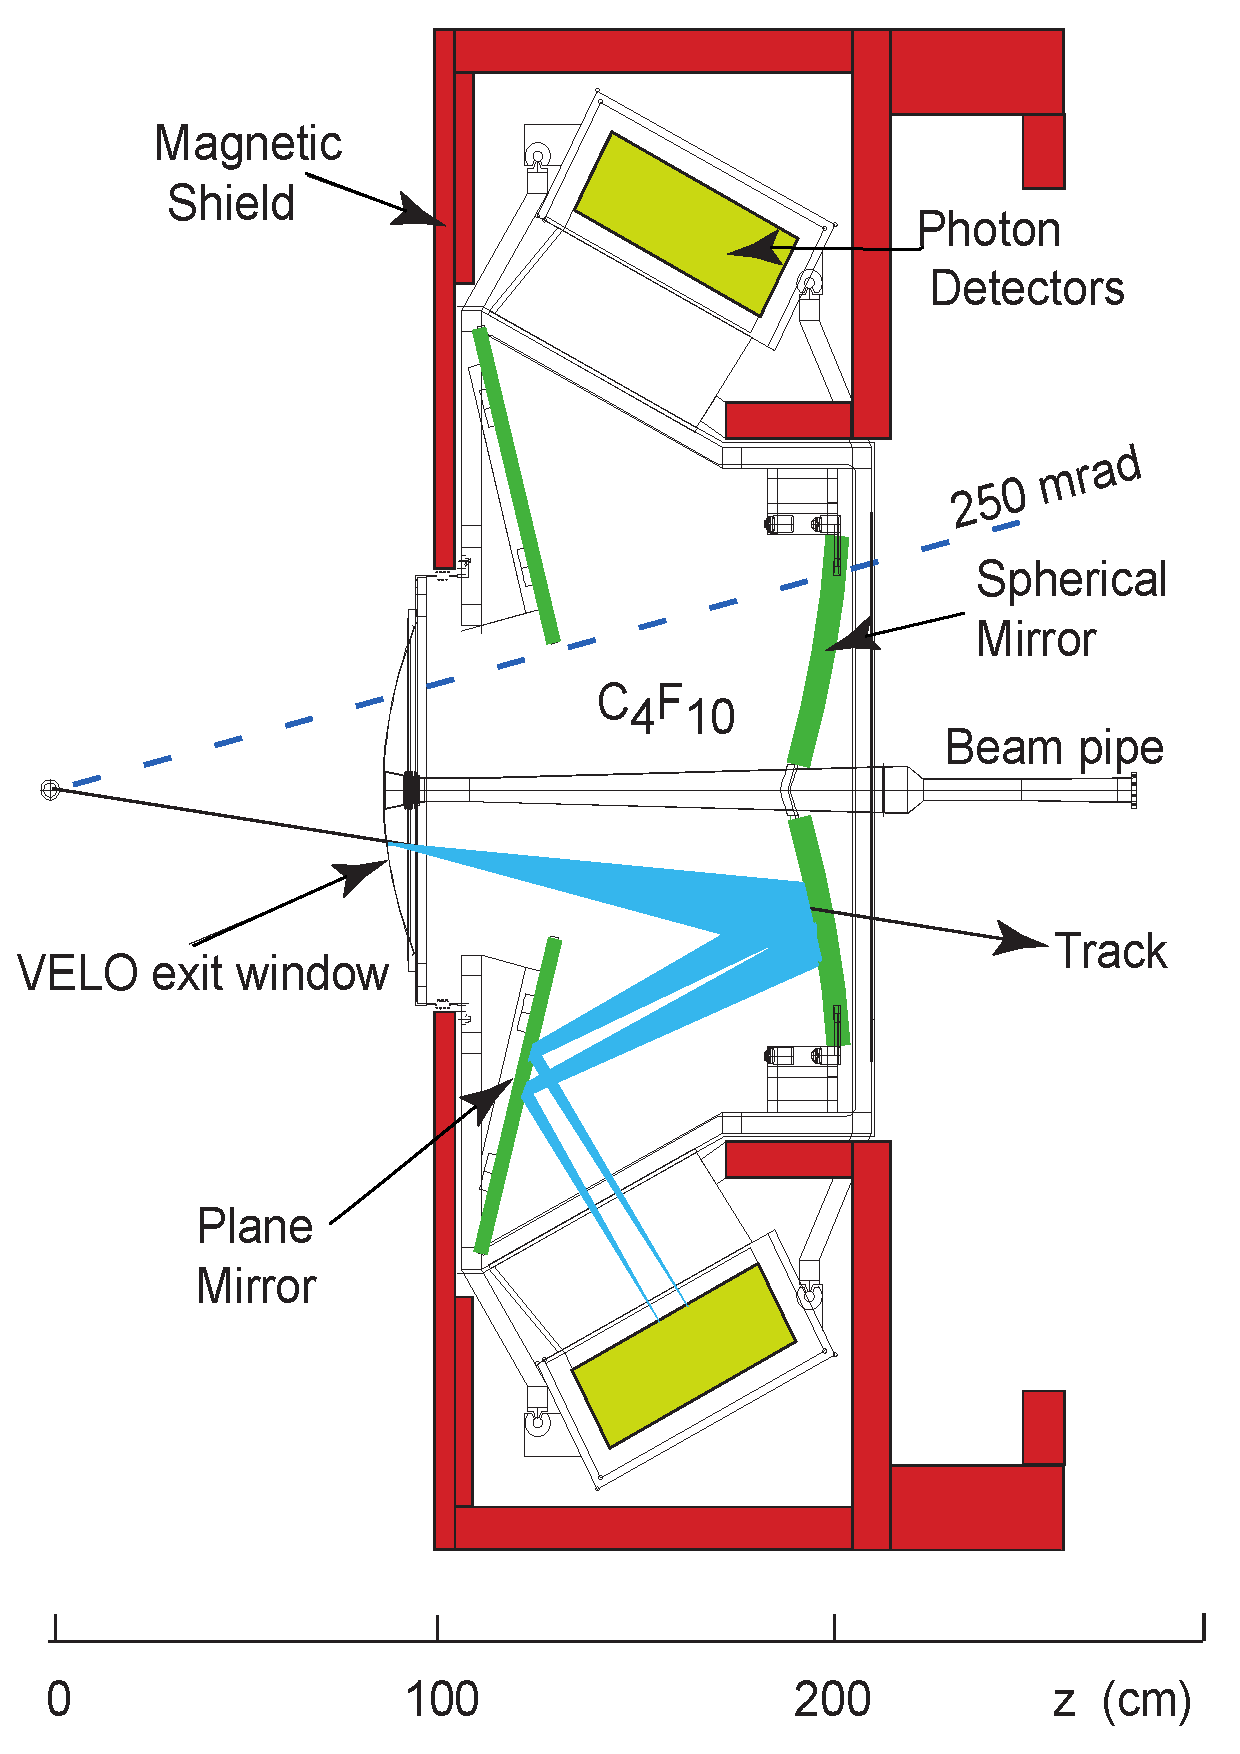
\includegraphics[width=0.49\textwidth,trim={0.0cm -0.45cm 0.0cm 0.0cm}]{figs/Introduction/rich1-2d-schematic.pdf}
    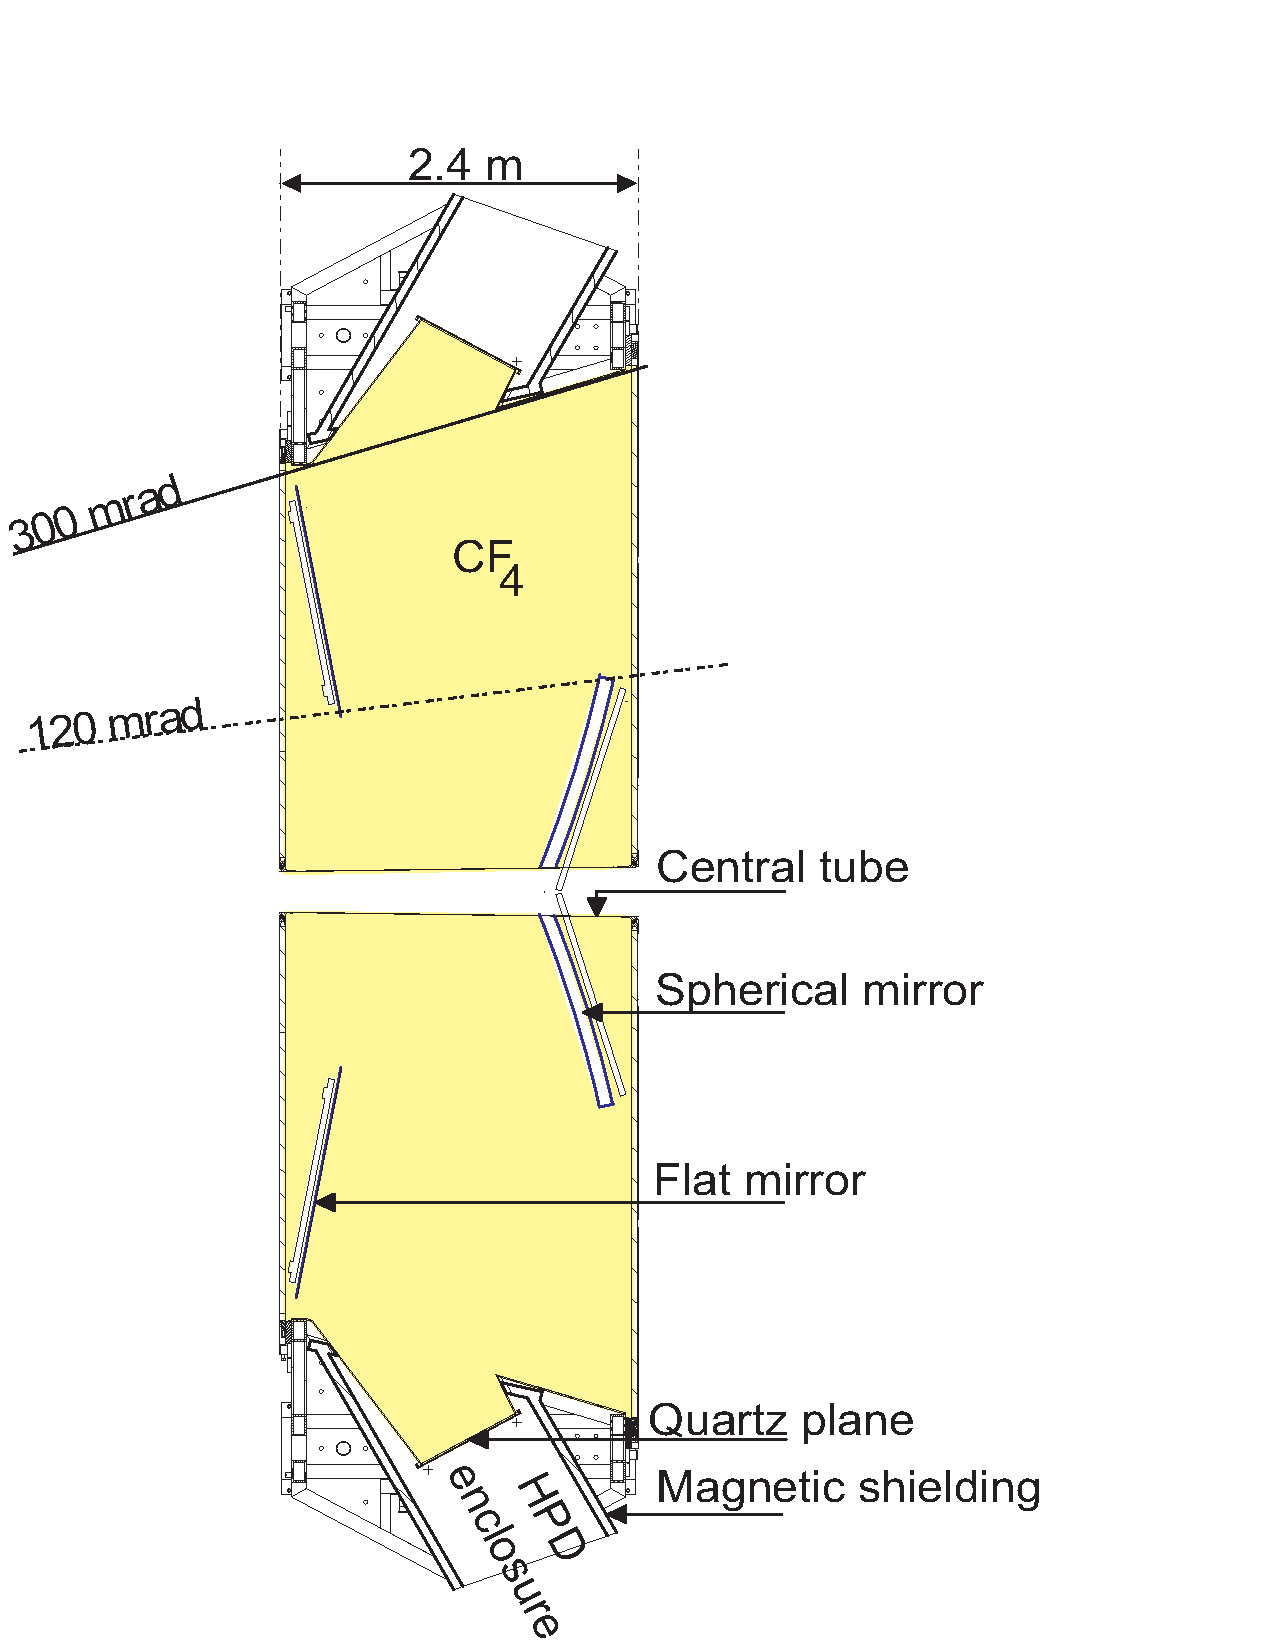
\includegraphics[width=0.49\textwidth,trim={0.0cm  0.0cm  3.5cm 2.5cm}]{figs/Introduction/RICH2_2d.pdf}
  }
  \hspace{0.51\textwidth}(a)\hspace{0.47\textwidth}(b)\hspace{0.02\textwidth}
  \vspace{-0.5\baselineskip}
  \caption{
    Schematic view of the LHCb RICH detectors and their optical systems:
    (a) side view of \richone and (b) top view of \richtwo. Formation of a
    Cherenkov ring in the lower part of \richone is also drawn.}
  \label{fig:RICH_OpticalLayout}
  \vspace{-0.5\baselineskip}
\end{figure}


The right-handed coordinate system of each mirror segment is defined by placing the origin at the centre of curvature with the $x$-axis pointing towards the mirror, the $y$-axis pointing upwards and the corresponding $z$-axis being horizontal. Finally, the pivot point for the software rotations around the $y$- and $z$-axes is at the centre of each mirror.\\
In order to achieve the optimal performance of the \lhcb \rich detector we aim to minimize the uncertainty, $\sigma$, associated with the measurement of a single photon Cherenkov angle. This is limited by four main sources of uncertainty outlined in Table \ref{tab:RichErrors}. Adding them in quadrature gives the minimal total uncertainty, which can be obtained by having an optimal alignment of all optical components of the \rich detectors.
\begin{table}[htb]
  \vspace{-0.5\baselineskip}
  \caption{
    Sources of uncertainty, $\sigma$, of the measurement of a single photon
    Cherenkov angle for the three \lhcb RICH radiators.}
  \vspace{-0.5\baselineskip}
  \centering
  \begin{tabular}{lcc}
                           &\multicolumn{2}{c}{$\sigma\,[\mathrm{mrad}]$}  \\
    \cmidrule(r){2-3}
                           &\richone&\richtwo  \\
    \cmidrule(r){2-3}
                            &   $\cfourften$   & $\cffour$\\
    \midrule
    \midrule
      Emission point        &      0.8         &     0.2  \\
      Chromatic dispersion   &      0.9         &     0.5  \\
      Pixel size            &      0.6         &     0.2  \\
      Tracking                &      0.4         &     0.4  \\
      \hline
      Total                &      1.5         &     0.7  \\
  \end{tabular}
  \label{tab:RichErrors}
  \vspace{-0.5\baselineskip}
\end{table}


%\section{HPD alignment}
\label{sec:HPDAlignment}


\section{Method of alignment for the RICH optical system}
\label{sec:MirrorAlignmentMethod}

An iterative, data-driven method for finding appropriate software compensations for the mirror misalignments was developed in the HERAb experiment~\cite{Gorisek:1999td}. The approach presented here builds on that method and is developed further to address the more complex design of the \lhcb \rich system.\\

A misalignment in the \lhcb \rich optical system manifests itself as a displacement of the observed Cherenkov ring against the expected one \cite{Papanestis:2008zz, Baldini:2006ed} as can be seen in Figure \ref{fig:RICH_MisalignmentDiagrams}. This can also be viewed as a discrepancy between the actual center of the Cherenkov ring - e.g. the center of the Cherenkov ring observed on the detector plane -  and its expected position calculated from the projection of the track onto the detector plane using the orientation of the optical components given in the current \lhcb conditions database. 

\begin{figure}[hbt]
  \vspace{-0.5\baselineskip}
  \centering{
    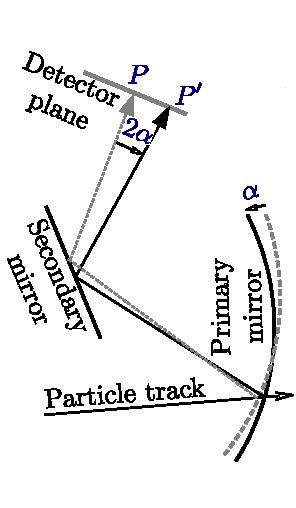
\includegraphics[width=0.27\textwidth]{figs/Method/TiltedMirror}
    \hspace{0.07\textwidth}
    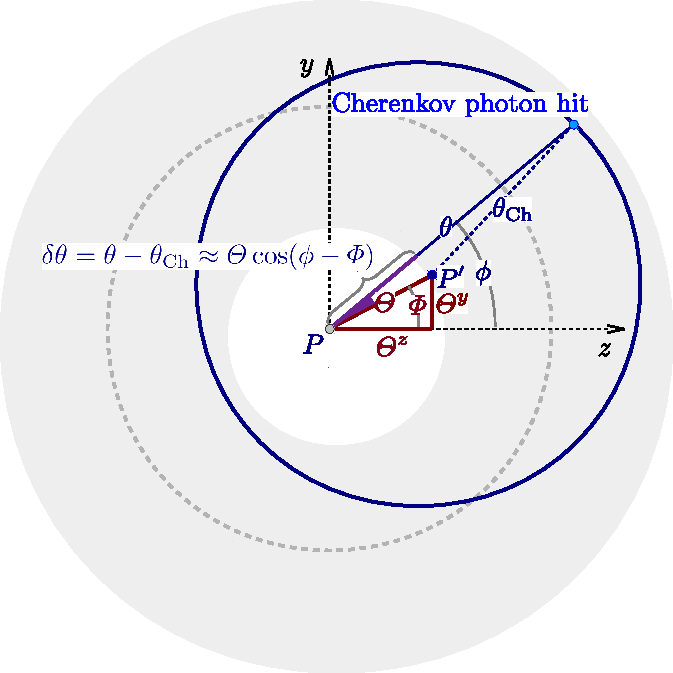
\includegraphics[width=0.61\textwidth]{figs/Method/ShiftedRing_andStripe}
  }
  \hspace{0.35\textwidth}(a)\hspace{0.52\textwidth}(b)\hspace{0.13\textwidth}
  \vspace{-0.5\baselineskip}
  \caption{
    (a) Schematic drawing of how a rotational misalignment of a \rich mirror (primary mirror in this example) causes shift of the actual centre $P'$ of the Cherenkov ring to $P$ on the photon detector plane. The projection of the track is drawn for explanatory purpose and represents the position of the expected centre of the Cherekov ring. (b) The expected Cherenkov angle \thetaC and the reconstructed Cherenkov angle $\theta$ are displayed. $P$ marks the position of the extrapolated track projection calculated without adjustments that would compensate any misalignments of the \rich mirrors, while $P'$ is the actual position of the centre of the ring and displaced by $\varTheta^z$ and $\varTheta^y$ with respect to $P'$ . Cherenkov angles $\theta$ are evaluated relative to $P$, and therefore, vary with $\phi$. The gray stripe represents area around the expected ring from which the photon hits are reconstructed. The width of this stripe is empirically chosen wide enough to cover the actual shifted (and somewhat smeared) ring of hits from a given track. Inevitably, the ``noise'' background photon hits in this area are also ``reconstructed''.}
  \label{fig:RICH_MisalignmentDiagrams}
  \vspace{-0.5\baselineskip}
\end{figure}

In order to observe and quantify the misalignment the quantity \deltatheta 
\begin{equation}
\delta\theta\left(\phi\right) = \theta\left(\phi\right) - \theta_{\mathrm{Ch}},
\end{equation}
-- where $\theta\left(\phi\right)$ is the the measured Cherenkov angle and $\theta_{\mathrm{Ch}}$ the expected Cherenkov angle -- is plotted against the azimuthal angle $\phi$ (see Figure \ref{fig:RICH_MisalignmentDiagrams}). For perfectly aligned mirrors \deltatheta is independent of $\phi$ but in case of a misalignment the distribution is approximately sinusoidal in $\phi$
\begin{equation}
  \label{eq:DeltaTheta_ps}
  \begin{aligned}
    \delta \theta_{p,s} (\phi) & \equiv   [\theta(\phi)-\theta_{\mathrm{Ch}} ]_{p,s}
                                 \approx  [\varTheta\cos(\phi-\varPhi)       ]_{p,s} \\
                               & =        [\varTheta\cos\varPhi\cos\phi
                                 +         \varTheta\sin\varPhi\sin\phi      ]_{p,s} \\
                               & =         \varTheta^z_{p,s}\cos\phi
                                 +         \varTheta^y_{p,s}\sin\phi                 \\
  \end{aligned}
\end{equation}
where the factors $\varTheta^y_{p,s}$ and $\varTheta^z_{p,s}$ represent the misalignments on the detector plane in $y$ and $z$ for a given mirror combination with primary mirror $p$ and secondary mirror $s$.\\
The misalignment factors $\varTheta^y_{p,s}$ and $\varTheta^z_{p,s}$ relate to the individual misalignments of the primary and secondary mirror via the \textit{magnification factors}
\begin{equation}
  \label{eq:theta0_y_z}
  \begin{aligned}
      A^y_{p,s}\alpha^y_p+B^y_{p,s}\beta^y_s
    + a^y_{p,s}\alpha^z_p+b^y_{p,s}\beta^z_s & = \varTheta^y_{p,s} \\
      A^z_{p,s}\alpha^z_p+B^z_{p,s}\beta^z_s
    + a^z_{p,s}\alpha^y_p+b^z_{p,s}\beta^y_s & = \varTheta^z_{p,s}
  \end{aligned}
\end{equation}
where $\alpha^y_p$, $\alpha^z_p$, $\beta^y_s$ and $\beta^z_s$ are the actual tilts of the primary and secondary mirrors around the $y$- and $z$-axis with respect to a given database. The magnification factors $A^y_{p,s}$, $B^y_{p,s}$, $a^y_{p,s}$ and $b^y_{p,s}$ ($A^z_{p,s}$, $B^z_{p,s}$, $a^z_{p,s}$ and $b^z_{p,s}$ for the $z$-axis) translate the effect of a tilt of the mirrors onto the detector plane (see Section \ref{subsec:Magnification}).\\
After all individual mirror tilts have been calculated a new database with the mirror orientations is created. It is useful to apply the alignment procedure iteratively to the same data sample, each time with the new database produced by the previous alignment. The alignment procedure is considered to have converged after no mirror has been found to have a misalignment greater than a chosen convergence criteria. \\
An overview of the entire alignment procedure can be seen in Figure \ref{fig:RICH_Procedure} while different details of the procedure are explained in the sections below.\\

\begin{figure}[h!]
  \centering{
    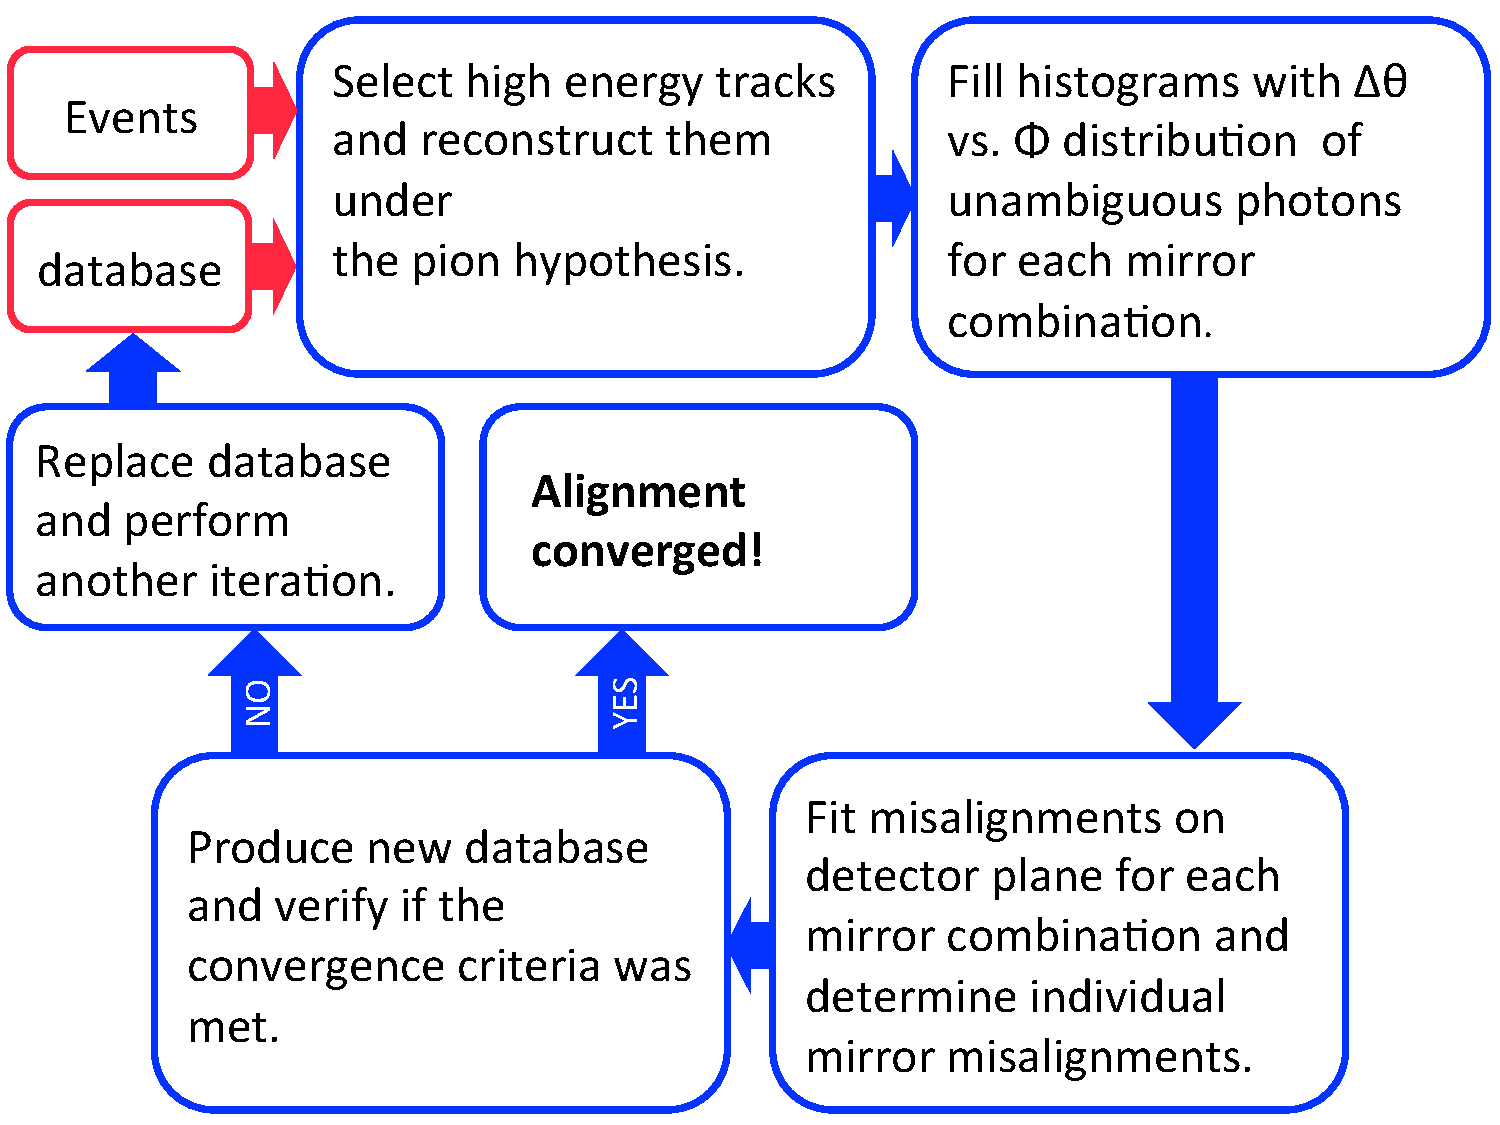
\includegraphics[width=0.7\textwidth]{figs/Method/procedure}
  }
  \vspace{-0.5\baselineskip}
  \caption{Overview of the entire alignment procedure. The alignment starts from a sample of events and usually from the mirror orientation given in the \lhcb conditions database. From there high energy tracks are reconstructed under the pion hypothesis (see Section \ref{subsec:TrackSelection}). Then the \deltatheta vs. $\phi$ histograms are filled for each mirror combination selected for the alignment procedure (see Section \ref{subsec:IndivMirrAlign}) and fitted to get the misalignments on the detector plane. With these the individual mirror misalignments are determined and a new database containing the corrected mirror orientations is created. If the convergence criteria is reached the alignment procedure is finished, if the criteria has not been reached the newly made database is used for the reconstruction of the same events and the entire procedure is repeated.}
  \label{fig:RICH_Procedure}
  \vspace{-0.5\baselineskip}
\end{figure}


\subsection{Track and photon selection}
\label{subsec:TrackSelection}
The events that the tracks and their photons are taken from are preselected. More information about the preselection and its implementation is given in Section \ref{sec:OnlineAlignmentFramework}.\\
In order to most accurately predict the Cherenkov angle for a given track some selection criteria are applied to the tracks themselves and to the photon candidates that make it into the \deltatheta vs. $\phi$ histograms.\\
High-momentum tracks are selected where the assumption can be made that the Cherenkov angle is saturated and therefore does not depend on the particle type any more. Figure \ref{fig:saturation} and Equation \ref{eq:DeltaTheta_ps} show the dependency of the Cherenkov angle of the momentum $p$ for different types of particles with mass $m$ in a radiator with refractive index $\eta$. 
\begin{equation}
  \label{eq:thetaC}
 \theta_{\mathrm{Ch}} = \arccos\left( \frac{1}{\eta} \sqrt{\left(\frac{m}{p}\right)^{2} + 1}  \right)
\end{equation}
In the case of high energy tracks all particles are assumed to have the the mass of a pion and the expected Cherenkov angle is calculated under that hypothesis.\\
\begin{figure}[htbp]
  \vspace{-0.5\baselineskip}
  \centering
  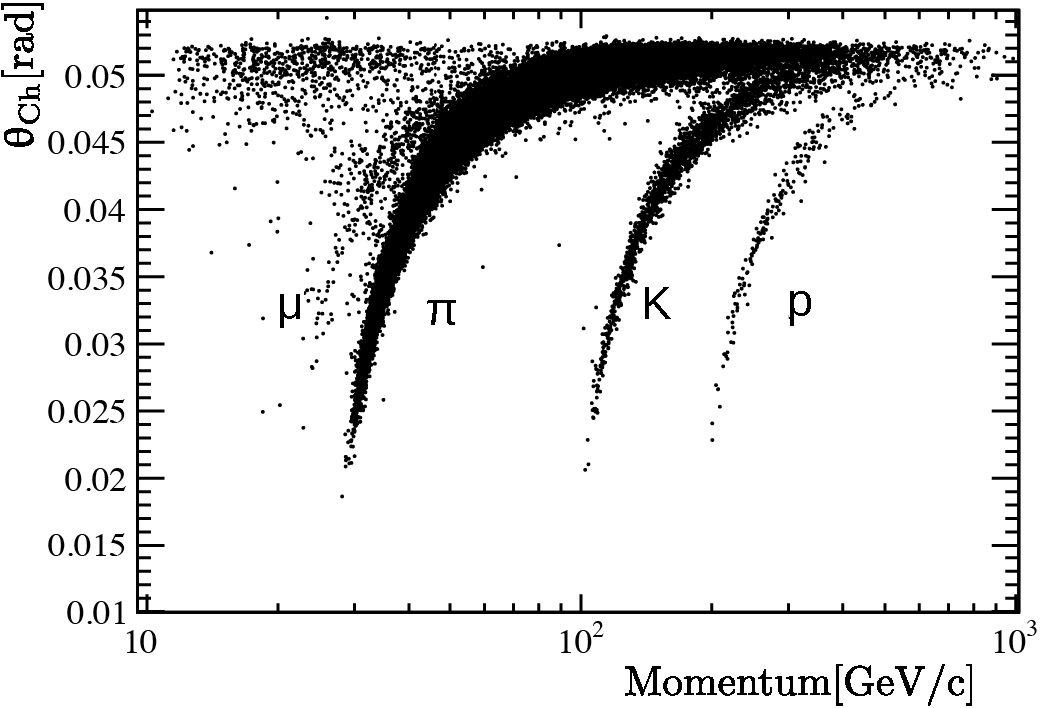
\includegraphics[width=0.75\textwidth]{figs/Method/ThetaVsMomentum_C4F10}
  \vspace{-0.5\baselineskip}
  \caption{
    Cherenkov angle \thetaC against track momentum, for tracks traversing the \richone gaseous radiator. Muons, pions, kaons and protons are visible. As the track momentum  increases, all particles tend towards the same \thetaC, known as the saturated Cherenkov angle.}
  \label{fig:saturation}
  \vspace{-0.5\baselineskip}
\end{figure}
The photon hits chosen to fill the \deltatheta vs. $\phi$ histograms are chosen from a ring-shaped area around the expected center of the Cherenkov ring (see Figure \ref{fig:RICH_MisalignmentDiagrams}). The ring's width is chosen to be big enough to cover the area of a shifted Cherenkov ring from a potentially misaligned mirror combination.\\
In the calculation of \deltatheta for the histograms the value for $\theta\left(\phi\right)$ is needed. This value is obtained by matching a photon hit on the detector plane to a track and calculating the Cherenkov angle. This requires an assumption about where along the track the Cherenkov photon was emitted. Since this is a intrinsically unknown quantity the assumption is made that the photon was emitted in the middle of the track. This introduces a source of noise from photons falsely associated with a given track. An analysis of MC events has shown~\cite{Gorisek:1999td} that it is possible to reduce this noise by only reconstructing \textit{unambiguous} photon hits. A photon hit is \textit{unambiguous} if it will be reflected by the same primary and secondary mirror independently of where along the particle track it was emitted. Therefore only unambiguous photon hits are chosen to be used in the alignment procedure in the \deltatheta vs. $\phi$ histograms.\\


\subsection{Method for fitting the \deltatheta vs. $\phi$ distributions}
\label{subsec:Fitting}

For every chosen combination of primary mirror $p$ and secondary mirror $s$, \deltatheta is plotted against $\phi$. Each of these two-dimensional distributions is divided into 20 bins in $\phi$. Inside each $\phi$ bin the \deltatheta distribution is fitted with a Gaussian plus a second order polynomial that represents the background photons. In accordance with Equation~\ref{eq:DeltaTheta_ps} the $\phi$ dependence of the position of the Gaussian peak for a given mirror combination $(p,s)$ is approximated by
\begin{equation}
  \label{eq:Delta_theta}
  \delta\theta_{p,s}(\phi) = \varTheta^z_{p,s}\cos\phi
                           + \varTheta^y_{p,s}\sin\phi.                         
\end{equation}
Equation~\ref{eq:Delta_theta} is used as a bond when fitting all the 20 slices jointly.\\
The fitting is done by means of the \root framework~\cite{Antcheva:2011zz}, in particular, using the \minuit minimization package. An example of a \deltatheta vs. $\phi$ histogram for a specific mirror combination in \richone, including the fitted sinusoidal of Equation \ref{eq:Delta_theta} is shown in Figure \ref{fig:Rich1Mirr0001dThetavphiRec}, before alignment and after the alignment.
\begin{figure}[htbp]
  \vspace{-0.5\baselineskip}
  \centering
  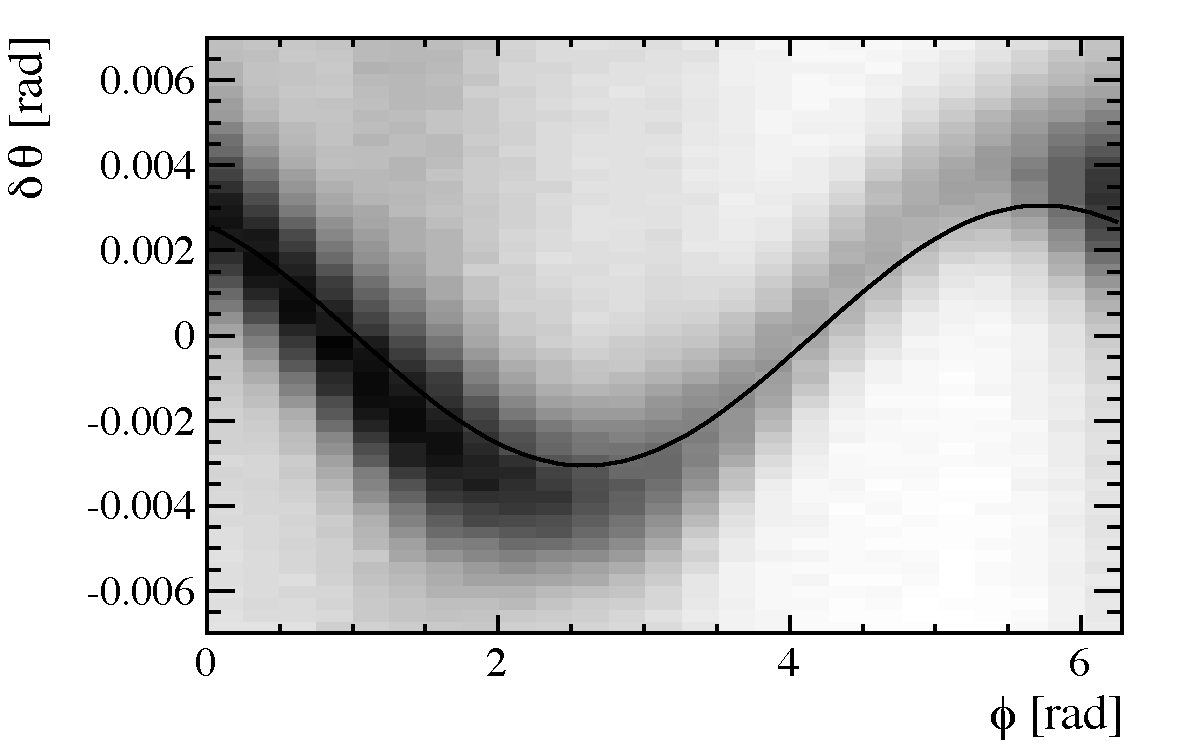
\includegraphics[width=.49\textwidth]
    {figs/Method/RICH1_ThetaVsPhiRec0001_misaligned.pdf}
  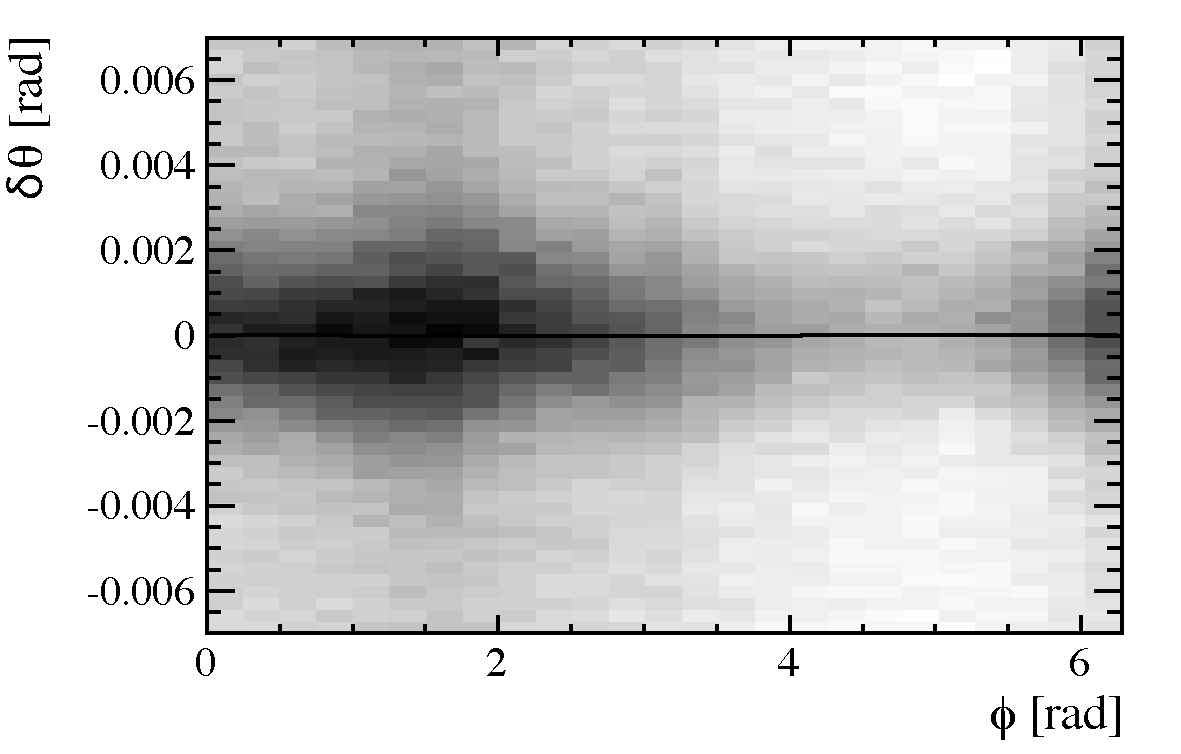
\includegraphics[width=.49\textwidth]
    {figs/Method/RICH1_ThetaVsPhiRec0001_aligned.pdf}
  \vspace{-1.0\baselineskip}
  \caption{
    \deltatheta against $\phi$ fitted slice-by-slice along $\phi$ with the function~\eqref{eq:Delta_theta} approximating the position of the Gaussian peaks on the $\phi\text{-}\delta\theta$~plane for the combination of primary mirror 0 and secondary mirror 1 of the \richone. The originally misaligned mirror combination is represented on the left while the right plot shows the same mirror combination after the alignment procedure.}
  \label{fig:Rich1Mirr0001dThetavphiRec}
  \vspace{-0.5\baselineskip}
\end{figure}


\subsection{Magnification factors}
\label{subsec:Magnification}
The magnification factors relate the tilts of the individual mirrors to the misalignment that can be observed in the detector plane. The effect of the magnification factors can be demonstrated in a simplified manner  by considering small rotations of primary and secondary mirrors around their $y$- axes. Those small rotations yield approximately the following displacement of the observable Cherenkov ring (as shown in~\fig{fig:RICH_MisalignmentDiagrams}):
\begin{equation}
l\,\varTheta^y \approx l_{\mathrm{pri}}2\,\alpha^y
                       - l_{\mathrm{sec}}2\, \beta^y,
\end{equation}
where $l$, $l_{\mathrm{pri}}$ and $l_{\mathrm{sec}}$ are lengths' of the paths of the photons to the photon detectors (from the emission point, from the primary mirror, and from the secondary mirror, respectively). Dividing this by the total photon path $l$ yields
\begin{equation}
\label{eq:magy}
  \varTheta^y  \approx \dfrac{2\,l_{\mathrm{pri}}}{l}\alpha^y
                     - \dfrac{2\,l_{\mathrm{sec}}}{l} \beta^y
               \approx                            A^y\alpha^y
                                                + B^y \beta^y
\end{equation}
where the factors in front of the actual mirror tilts $\alpha^y$ and $\beta^y$ are defined to be the magnification factors. The above equation is for illustrative purposes only and represents a simplified view because is doesn't take effects from rotations around the alternative (here $z$-) axis into account. The full expression used in the alignment procedure is shown in Equation \ref{eq:theta0_y_z}.\\
The magnification factors are determined using a data-driven method. Eight independent calibrational rotations (positive/negative rotations about the $y$- / $z$- axis for the primary and secondary mirrors) are introduced. Then the resulting misalignment on the detector plane is measured and used to solve Equation \ref{eq:magy} for the magnification factors. The final value of each magnification factor is arithmetical mean of the two corresponding values obtained with the calibrational rotations in opposite directions.\\
The size of each calibrational rotation for \richone is chosen to be $\pm0.7\mrad$ in order to sufficiently determine the magnification factors. This choice is motivated by the fact that the Cherenkov angle resolution for \richone is around $1.6\mrad$. Due to the smaller resolution of $0.7\mrad$ in \richtwo, the size of its calibrational rotations is chosen to be $\pm0.3\mrad$.\\


\subsection{Determining individual mirror misalignments}
\label{subsec:IndivMirrAlign}
The fits to the \deltatheta vs. $\phi$ distributions yield the misalignments in $y$ and $z$ on the detector plane for a given mirror combination. In order to determine the actual positioning of the mirrors for the \lhcb conditions database, the misalignments of the individual primary and and secondary mirrors are needed. This gives a system with more unknowns (individual mirror misalignments in $y$ and $z$) than equations. However, an optimal alignment can be achieved if each component of the optical system is properly aligned relative to all others. Therefore all mirrors only need to be aligned with respect to each other.\\


\subsubsection{\richone alignment}
\label{subsec:Rich1Align}

The geometry of the \lhcb \richone detector restricts the number of populated mirror combinations to 16, as shown in Figure \ref{fig:RICH1_MirrorNumbering}. Photons reflected off a primary mirror are reflected off one of four secondary mirrors that form a group, unique to that primary mirror. Each of the four quadrants contain a single primary mirror and four secondary mirrors.
\begin{figure}[htbp]
  \vspace{-0.5\baselineskip}
  \centering
  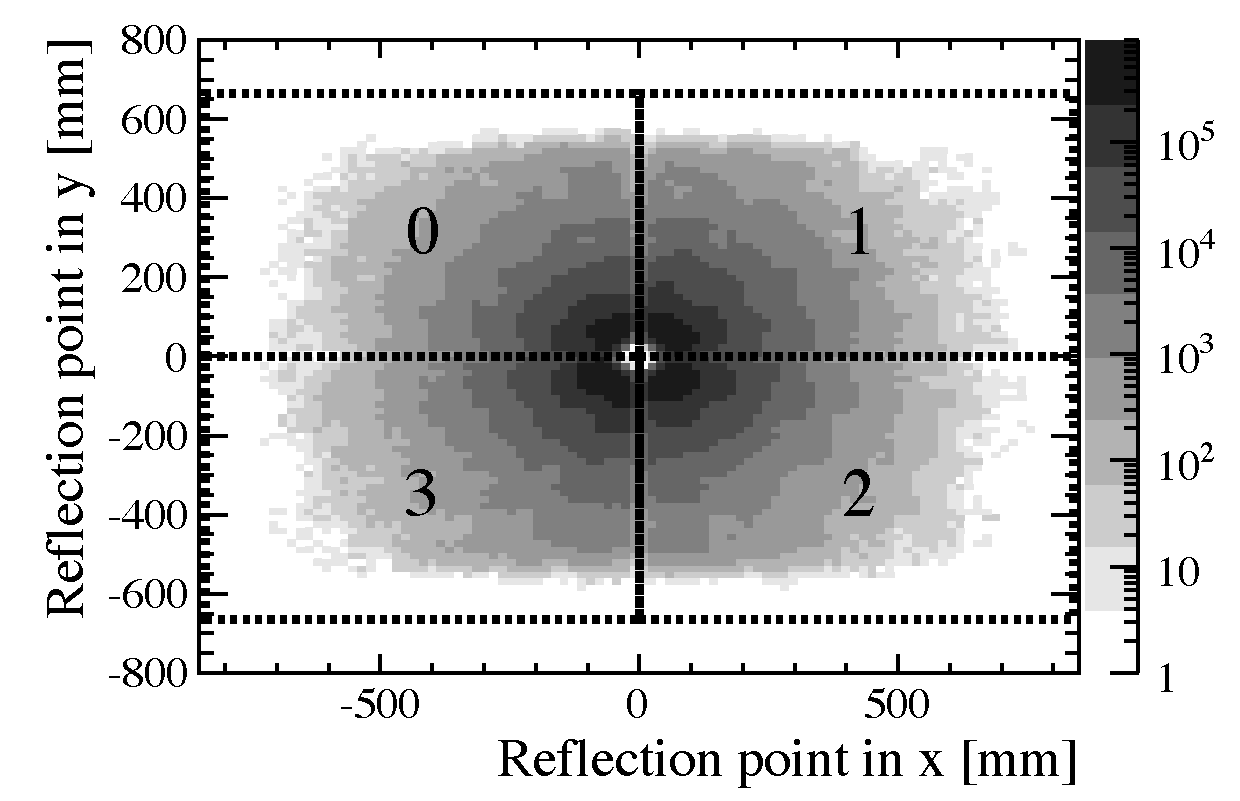
\includegraphics[width=.48\textwidth]{figs/Method/RICH1_PrimaryMirrors.pdf}
  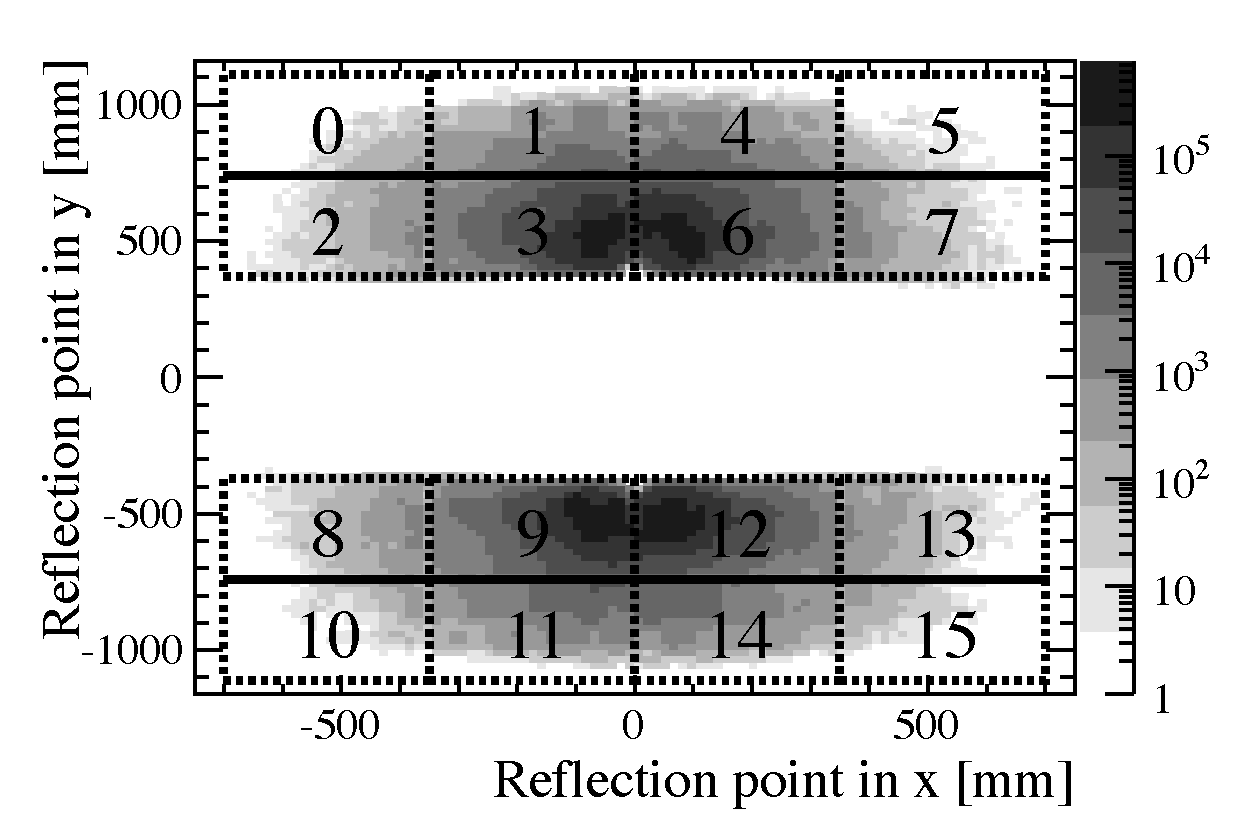
\includegraphics[width=.48\textwidth]{figs/Method/RICH1_SecondaryMirrors.pdf}
  \vspace{-0.5\baselineskip}
  \caption{
    \richone mirror numbering scheme and reflection point distribution of photons off \richone primary mirrors (left) and secondary mirrors (right). The photon population across mirrors is not uniform with the higher populated mirrors laying closest to the beam-pipe.}
  \label{fig:RICH1_MirrorNumbering}
  \vspace{-0.5\baselineskip}
\end{figure}

Thus for each quadrant there are four equations and five unknowns for the $y$- and $z$-direction respectively. These are shown here for the example of the quadrant of primary number 0 in the $y$-direction

\begin{equation*}
  \label{eq:zeroQuadrantMirrorTilts}
  \arraycolsep=1pt
  \begin{array}{*{5}c}
    A^y_{0,0}\alpha^y_0 & + & B^y_{0,0}\beta^y_0 & = & \varTheta^y_{0,0} \\
    \vdots              &   & \vdots             &   & \vdots \\
    A^y_{0,3}\alpha^y_0 & + & B^y_{0,3}\beta^y_3 & = & \varTheta^y_{0,3}.
  \end{array}
\end{equation*}

Since the mirrors only need to be aligned with respect to each other the primary mirrors are excluded from the adjustment procedure, i.e. it is assumed that $\alpha^y_0=0$. The misalignment of the secondary mirrors are directly calculated from $\beta^y_s=\varTheta^y_{0,s}/B^y_{0,s}$ and thus contain a compensation for the misalignment of their respective primary mirrors.


\subsubsection{\richtwo alignment}

The geometrical layout of the \richtwo detector is significantly different to that of \richone in that a given primary mirror can reflect photons onto several secondary mirrors and a given secondary mirror can receive photons from different primary mirrors. The mirrors can only be divided into two decoupled systems: 48 mirrors on the left side of the beam, and 48 mirrors on the right side  of the beam as can be seen in Figure \ref{fig:RICH2_MirrorNumbering}. This gives 96 unknown parameters for each side (tilts around $y$- and $z$- axes for each mirror) from which only 47 out of the 48 possible tilts are independent, since a simultaneous rotation of all primary mirrors by one angle and all secondary mirrors by the corresponding angle in the opposite direction will not change the position of the Cherenkov ring on the detector plane.\\
Each mirror only reflects/receives photons onto/from a couple of adjacent mirrors of the opposite kind. Thus there are still many more unknowns than there are equations. As for \richone the fact is used that all mirrors only have to be adjusted with respect to each other. For \richtwo that means that for each side one mirror is chosen to stay fixed while all other mirrors are aligned with respect to it by a chain of equations linking all mirrors together. There are different possibilities of connecting all mirrors and the one chosen for the alignment procedure is the one that maximises the number of photons exchanged between mirrors. The way the mirrors are chosen to be linked for the left half of \richtwo can be seen in Figure \ref{fig:RICH2_MirrorLinking}. Additionally the involved mirror combinations are listed in Tables \ref{tab:ChosenConbinationsPri} and \ref{tab:ChosenConbinationsSec} grouped by primary and secondary mirrors respectively.\\
The result is a system of 94 linear equations (47 combinations of Equations \ref{eq:theta0_y_z}) which is solved algebraically using the substitution method between different mirror combinations and Cramers's rule within the two equations for one mirror combination.\\
\begin{figure}[htbp]
  \vspace{-0.5\baselineskip}
  \centering
  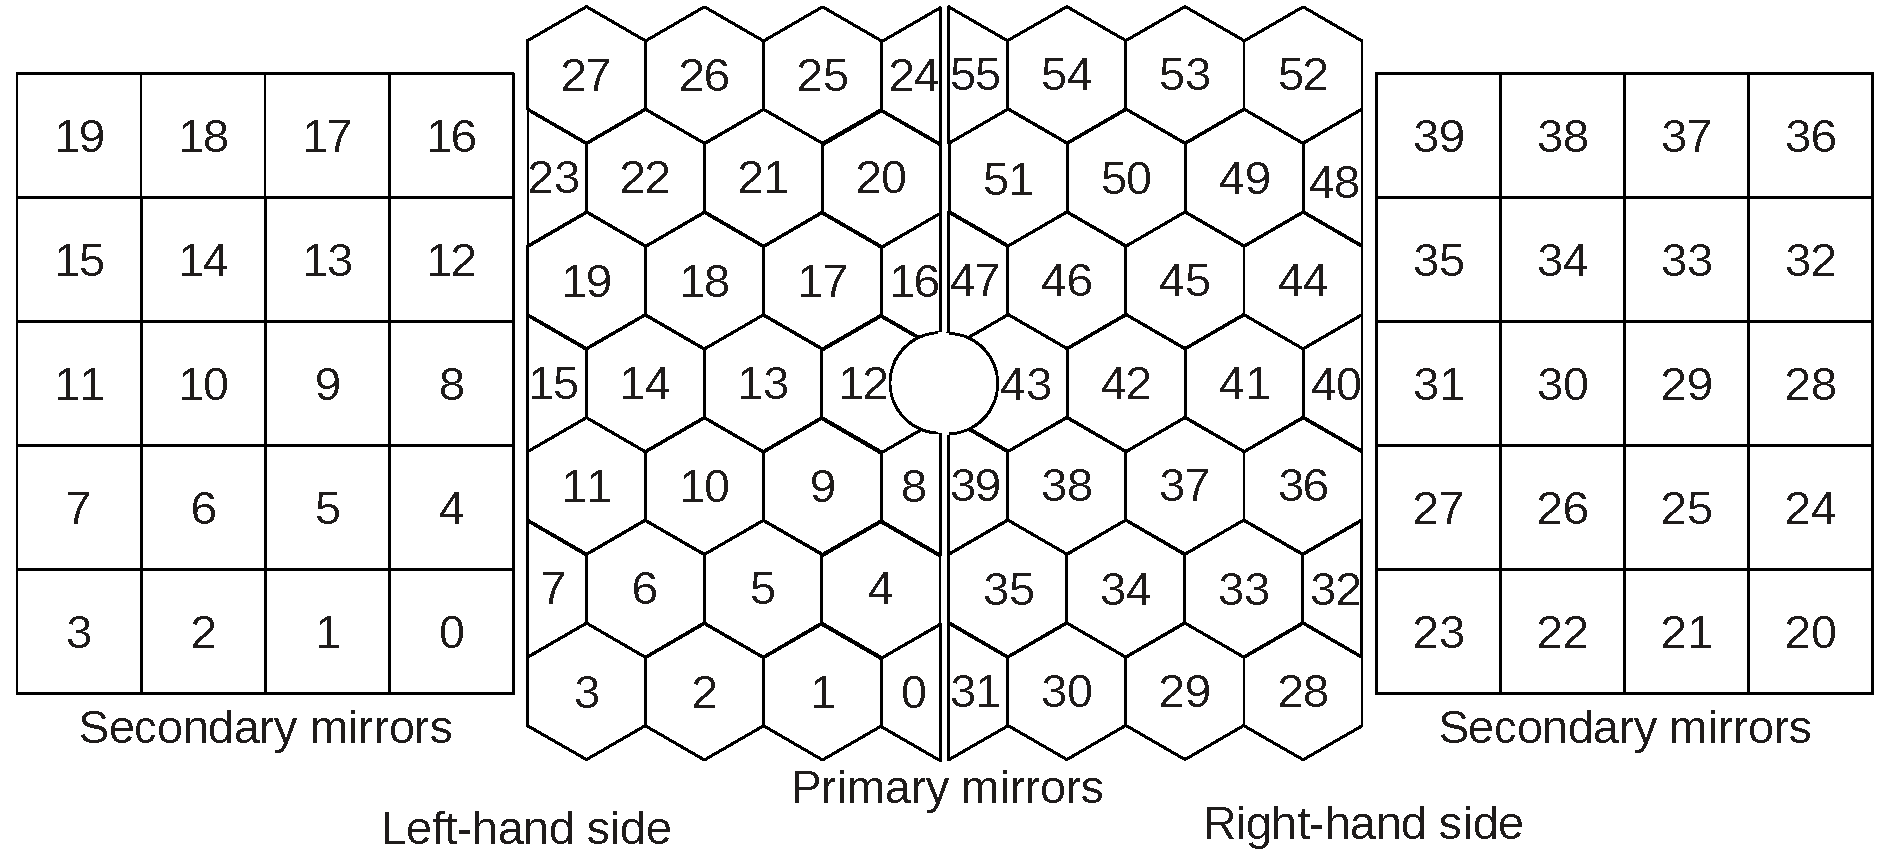
\includegraphics[width=\textwidth]{figs/Method/RICH2_MirrorNumberingBothSides.pdf}
  \vspace{-1.0\baselineskip}
  \caption{ \richtwo mirror segmentation numbering scheme, viewed along the beam with the beampipe at the center.}
  \label{fig:RICH2_MirrorNumbering}
  \vspace{-0.5\baselineskip}
\end{figure}


\begin{figure}[htbp]
  \vspace{-0.5\baselineskip}
  \centering
  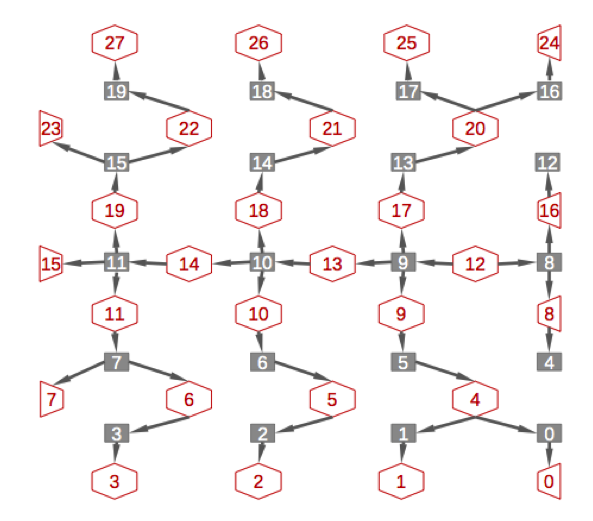
\includegraphics[width=0.5\textwidth]{figs/Method/MirrorLinking.png}
  \vspace{-1.0\baselineskip}
  \caption{ Illustration of how the primary and secondary mirrors of the left half of \richtwo are linked in order to align them with respect to each other starting by fixing  primary mirror 12.}
  \label{fig:RICH2_MirrorLinking}
  \vspace{-0.5\baselineskip}
\end{figure}

\setlength{\tabcolsep}{6pt}
\newcolumntype{d}[1]{ D{,} {,} {#1} }

\begin{table}[htb]
  \caption{
    The 47 chosen $p,s$ (primary,secondary) mirror combinations grouped by primary mirror for the left-hand side of \richtwo.}
  \vspace{-0.5\baselineskip}
  \centering
 %\scriptsize
  \small
  \sffamily
  \begin{tabular}{*{4}{|d{2}d{2}}|}
    \hline
           & 27,19 &       & 26,18 &       & 25,17 &       & 24,16 \\
    \hline
           &       & 22,19 & 22,18 &       & 21,17 &       & 20,16 \\
           & 23,15 &       & 22,14 &       & 21,13 &       & 20,12 \\
    \hline
           & 19,15 &       & 18,14 &       & 17,13 &       & 16,12 \\
           & 19,11 &       & 18,10 &       & 17,9  &       & 16,8  \\
    \hline
           & 15,11 & 14,11 & 14,10 & 13,10 & 13,9  & 12,9  & 12,8  \\
    \hline
           & 11,11 &       & 10,10 &       &  9,9  &       &  8,8  \\
           & 11,7  &       & 10,6  &       &  9,5  &       &  8,4  \\
    \hline
           &  7,7  &       &  6,6  &       &  5,5  &       &  4,4  \\
           &       &  6,3  &  6,2  &       &  5,1  &       &  4,0  \\
    \hline
           &  3,3  &       &  2,2  &       &  1,1  &       &  0,0  \\
    \hline
  \end{tabular}
  \label{tab:ChosenConbinationsPri}
  \vspace{-0.5\baselineskip}
\end{table}

\begin{table}[htb]
  \caption{
    The 47 chosen $p,s$ (primary,secondary) mirror combinations grouped by secondary mirrors for the left-hand side of \richtwo.}
  \vspace{-0.5\baselineskip}
  \centering
 %\scriptsize
  \small
  \sffamily
  \begin{tabular}{*{4}{|d{2}d{2}}|}
    \hline
           & 27,19 &       & 26,18 &       & 25,17 &       & 24,16 \\
           & 22,19 &       & 22,18 &       & 21,17 &       & 20,16 \\
    \hline
           & 23,15 &       & 22,14 &       & 21,13 &       & 20,12 \\
           & 19,15 &       & 18,14 &       & 17,13 &       & 16,12 \\
    \hline
           & 19,11 &       & 18,10 &       & 17,9  &       & 16,8  \\
     15,11 & 14,11 & 14,10 & 13,10 & 13,9  & 12,9  &       & 12,8  \\
           & 11,11 &       & 10,10 &       &  9,9  &       &  8,8  \\
    \hline
           & 11,7  &       & 10,6  &       &  9,5  &       &  8,4  \\
           &  7,7  &       &  6,6  &       &  5,5  &       &  4,4  \\
    \hline
           &  6,3  &       &  6,2  &       &  5,1  &       &  4,0  \\
           &  3,3  &       &  2,2  &       &  1,1  &       &  0,0  \\
    \hline
  \end{tabular}
  \label{tab:ChosenConbinationsSec}
  \vspace{-0.5\baselineskip}
\end{table}


\section{The Online Alignment Framework}
\label{sec:OnlineAlignmentFramework}

\subsection{Dataflow in Run II}
\label{subsec:Dataflow}
The \lhcb trigger strategies for the Run I and Run II data taking periods are shown in Figure \ref{fig:dataflow}.\\
In Run I the online event reconstruction was simpler and faster than the reconstruction used offline and did not include any information about the particle identification (PID). In order to have the same reconstruction online and offline as well as using the PID information in the \hlttwo the data-taking strategy has been amended for Run II. As in Run I a rate of 1\mhz of events passes the level-0 trigger (\lone) and is passed on to the first high level trigger stage (\hltone). There the events are partially reconstructed and accepted events are written to disk. At this stage the different alignments are run on a dedicated part of the buffered data. In case of a big shift in alignment constants the new constants are propagated to the \lhcb conditions database and used in the subsequent processing of the events by the second high level trigger (\hlttwo).\\
The alignment tasks being performed on the data are - in the order they are being run - \velo alignment, tracker alignment, \rich alignment and finally muon chamber alignment. Each alignment has its own dedicated \hltone line which collects a given number of events at the beginning of each fill (see Section \ref{subsec:HltForRich} for the \rich lines). It has been found that $\sim$1 \m events for \richone and $\sim$2\m events for \richtwo is sufficient to produce stable results. Once enough events have been collected the alignment is started.\\
\begin{figure}[htbp]
  \vspace{-0.1\baselineskip}
  \centering
  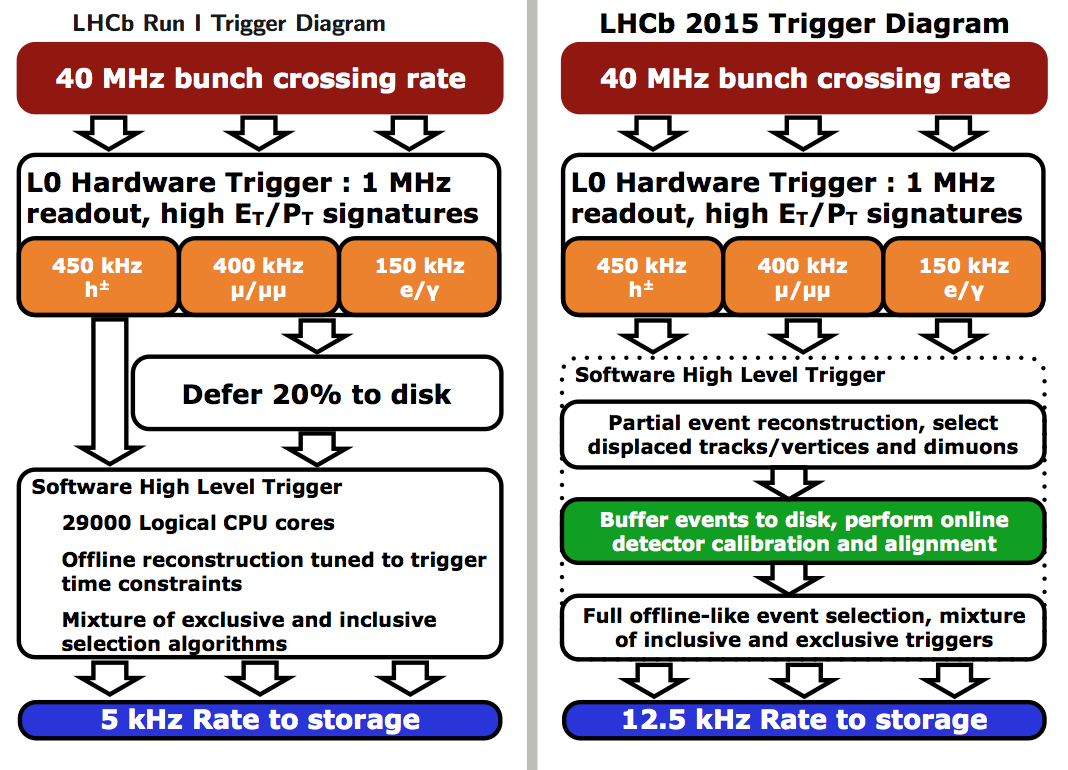
\includegraphics[width=0.75\textwidth]{figs/Online/dataflow}
  \vspace{-0.5\baselineskip}
  \caption{\lhcb dataflow for Run I (left) and Run II (right). In Run II the data is buffered after \hltone and an alignment is performed for each fill. The \hlttwo will then process the buffered events with the updated alignment constants.}
  \label{fig:dataflow}
  \vspace{-0.5\baselineskip}
\end{figure}


\subsection{\hltone selection for the \rich mirror alignment}
\label{subsec:HltForRich}
In order to determine the misalignments on the detector plane and subsequently the individual mirror misalignments the \deltatheta vs. $\phi$ histograms for each mirror combination have to contain enough entries for the fits described in Section \ref{subsec:Fitting} to converge. The minimum condition for a successful fit has been found to be that 16 of the 20 bins in $\phi$ have to contain at least 300 entries.\\
This is accomplished by having two dedicated \hltone selections, one each for \richone and \richtwo. The lines trigger on high energy particle tracks whose Cherenkov photons would populate the mirror combinations containing the fewest photons. The other mirror combinations are then populated by the rest of the tracks in the events.\\
The variables used in the selection are the track momentum $p$, the transverse track momentum $p_T$, the pseudorapidity $\eta$, the goodness of fit for the track $\chi^2$ and the polar angle of the track $\phi$. The selection criteria of tracks that are triggered upon are listed in Table \ref{tab:HltCuts}. \\

\begin{table}[htb]
  \vspace{-0.5\baselineskip}
  \caption{Trigger criteria for the \hltone line for \richone and \richtwo. Events that are accepted by these trigger lines need to have at least one track that satisfies the cuts listed below.}
  \vspace{-0.5\baselineskip}
  \centering
  \begin{tabular}{l|c|c}
  & \richone & \richtwo \\
  \hline
  momentum $p$ & $p>20$ \gev & $p>40$ \gev \\
  \hline
  transverse momentum $p_T$ & $p_T > 0.5$ \gev & $p_T > 0.5$ \gev \\
  \hline
  pseudorapidity $\eta$ & $1.6< \eta <2.04$ & $ 2.65 <\eta < 2.80 $\\
  \hline
  track $\chi^2$ & $\chi^2 < 2$ & $\chi^2 < 2$ \\
  \hline
  polar angle $\Phi$ & $-2.65< \Phi <-2.30$ & $-2.59< \Phi <-2.49$ \\
   & $-0.80 < \Phi <-0.50 $ & $-0.65 < \Phi <-0.55 $ \\
   & $0.50 < \Phi < 0.80$ & $ 0.55 < \Phi < 0.65 $ \\
   &  $ 2.30 < \Phi <2.65 $ & $2.49 < \Phi < 2.59 $ \\
  \end{tabular}
  \label{tab:HltCuts}
  \vspace{-0.5\baselineskip}
\end{table}

\subsection{The Alignment Farm}
\label{subsec:AlignmentFarm}
All alignments are run on the alignment farm. The alignment farm consists of approximately 1700 CPUs, called \textit{analysers} and a central node called the \textit{iterator}.\\
The data taken from the \hltone selection for the \rich alignments is stored evenly distributed over the analysers until it can be processed by \hlttwo. The analysers perform the event reconstruction with a database provided to them by the iterator and fill the \deltatheta vs. $\phi$ histograms mentioned in Section \ref{sec:MirrorAlignmentMethod}. Apart from providing the database with the desired mirror orientations the iterator also performs the fits on the histograms, determines the individual mirror misalignments, produces a new database and decides whether the alignment procedure has converged or whether another iteration has to be performed. If the latter is the case, the iterator will make the new database available to the analysers (for more details see Section \ref{subsec:implementation}).\\
The advantage of having a system consisting of about 1700 nodes distributed over 50 farms is that the event reconstruction can happen in parallel and is therefore very fast. This parallel processing is asynchronous and has to be coordinated between the individual analysers and the iterator which is described in the next section.\\


\subsection{The Control Flow}
The execution of the alignment tasks is under the control of the LHCb Experiment Control System (ECS), and is implemented as a \textit{finite state machine}, which is illustrated in Figure \ref{fig:states}. The principle of a finite state machine means that each component of the system (here every individual analyser and the iterator) has to be in one of a finite number of states at all times. The states used for the alignment procedure are also shown in Figure \ref{fig:states}, such as ``READY'', ``RUNNING'' and ``PAUSED''. The alignment is then steered by the \textit{run control} that can see all the components and their individual states and can send commands. Those commands will be received by the individual components and they will act accordingly. For a given state only a certain number of commands are possible - for example if the component is in state ``PAUSED'' it can only receive the commands ``continue'' and ``stop''. If a command is received the component will go from its state into the state declared by Figure \ref{fig:states}. When in a new state the component will usually perform a task and then set itself into another state once finished so that the run control is aware of this task being completed.\\ 

\begin{figure}[htbp]
  \vspace{-0.5\baselineskip}
  \centering
  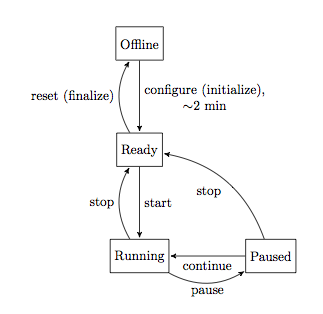
\includegraphics[width=0.7\textwidth]{figs/Online/states}
  \vspace{-0.5\baselineskip}
  \caption{Example of one component within a system functioning under the principle of a finite state machine. The boxes show the states the component is in while the arrows show the commands the component gets from the run control.}
  \label{fig:states}
  \vspace{-0.5\baselineskip}
\end{figure}


\subsection{Implementation of the \rich Mirror Alignment for Run II}
\label{subsec:implementation}
The interplay between the iterator, one example analyser and the run control during the course of the alignment of a \rich detector is shown in Figure \ref{fig:runcontrol}.\\
The individual analysers and the iterator all follow the same sequence of states, namely the one shown in Figure \ref{fig:states}. When the alignment is being started the run control sends the command to ``configure'' to both the iterator and all analysers. All components will go into state ``CONFIGURING'' while setting up to run the alignment. For the analysers this means that they read in the configuration for the reconstruction of the events, while the iterator sets up a directory in which all files for this alignment are saved.\\
Each component goes into state ``READY'' when it is done configuring. When all tasks are in the ``READY'' state, the iterator makes an initial set of alignment constants available to the analysers and then updates its state to ``RUNNING''. The analyzers are then sent the``start'' command, update their state to ``RUNNING'' and start reconstructing the data stored on them. Each analyser that has completed processing its data updates its state to ``PAUSED'', and once they have all reached this state, the run control sends the “stop” command and they update their states to ``READY''. The iterator is then sent the ``pause'' command, collects and combines the histograms produced by the analyser tasks and performs the fits. It then calculates the individual mirror misalignments and produces a new database containing the mirror orientations. The it either indicates that conversion has been reached by updating its state to ``READY'', or that further iteration is required by updating its state ``RUNNING''. In the latter case the iterator will provide the new database to the analysers before changing its state and another iteration is started.\\

\begin{figure}[htbp]
  \vspace{-0.5\baselineskip}
  \centering
  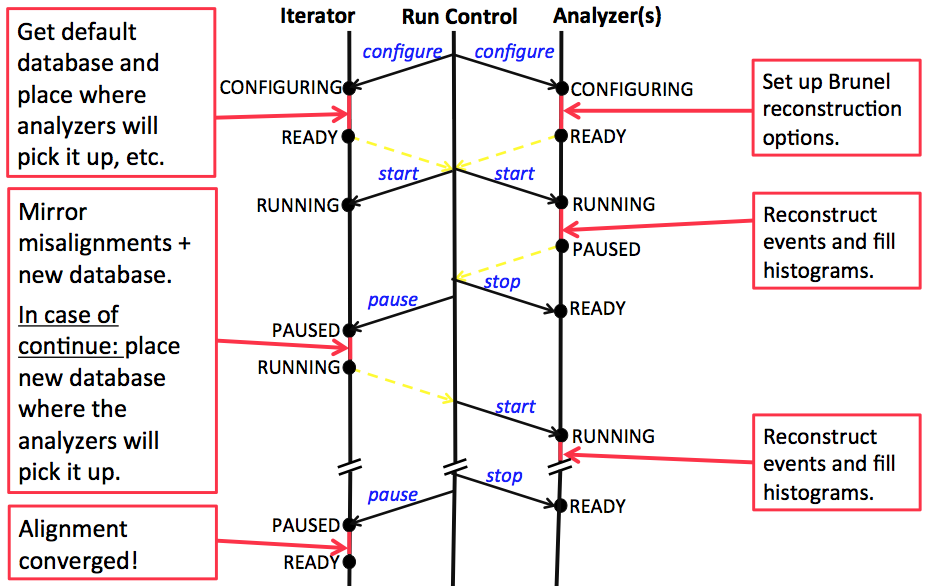
\includegraphics[width=\textwidth]{figs/Online/runcontrol}
  \vspace{-0.5\baselineskip}
  \caption{Interplay between the iterator, one example analyser and the run control during the \rich alignment procedure. The analysers reconstruct the data and produce the histograms that the iterator evaluates. The run control makes sends commands to the iterator and the analysers to make sure the alignment procedure happens in the necessary sequence. }
  \label{fig:runcontrol}
  \vspace{-0.5\baselineskip}
\end{figure}

%\section{Event selection}
\label{sec:SelectionMethod}
In order to determine the misalignments on the detector plane and subsequently the individual mirror misalignments the \deltatheta vs. $\phi$ histograms for each mirror-pair have to contain enough entries for the fits described in Section \ref{subsec:Fitting} to converge. The condition for a successful fit has been found to be that 16 of the 20 bins in $phi$ have to contain at least 300 entries.\\
This is accomplished by having two dedicated \hltone lines for \richone and \richtwo respectively. The lines trigger on high energy particle tracks whose Cherenkov photons would populate the mirror-pairs containing the outer primary mirrors. (These mirror-pairs have lowest occupancy during normal data-taking since the particle flow is greatest close to the beam-pipe.) The other mirror-pairs are then populated by the rest of the tracks in the events. The selection criteria of tracks that are triggered on are listed in Table \ref{tab:HltCuts}. \\

\begin{table}[htb]
  \vspace{-0.5\baselineskip}
  \caption{Trigger criteria for the \hltone line for \richone and \richtwo. Events that are accepted by these trigger lines need to have at least one track that satisfies the cuts listed below.}
  \vspace{-0.5\baselineskip}
  \centering
  \begin{tabular}{l|c|c}
  & \richone & \richtwo \\
  \hline
  momentum $p$ & $p>20$ \gev & $p>40$ \gev \\
  \hline
  transverse momentum $p_T$ & $p_T > 0.5$ \gev & $p_T > 0.5$ \gev \\
  \hline
  pseudorapidity $\eta$ & $1.6< \eta <2.04$ & $ 2.65 <\eta < 2.80 $\\
  \hline
  track $\chi^2$ & $\chi^2 < 2$ & $\chi^2 < 2$ \\
  \hline
  polar angle $\Phi$ & $-2.65< \Phi <-2.30$ & $-2.59< \Phi <-2.49$ \\
   & $-0.80 < \Phi <-0.50 $ & $-0.65 < \Phi <-0.55 $ \\
   & $0.50 < \Phi < 0.80$ & $ 0.55 < \Phi < 0.65 $ \\
   &  $ 2.30 < \Phi <2.65 $ & $2.49 < \Phi < 2.59 $ \\
  \end{tabular}
  \label{tab:HltCuts}
  \vspace{-0.5\baselineskip}
\end{table}


%\section{Computing framework}
\label{sec:Framework}

A computing framework that automates the \rich mirror software alignment
procedure was developed. It is based on \ganga~\cite{Mościcki20092303}, a tool
for computational-task management and easy access to Grid resources. A schematic
workflow diagram is shown in \fig{fig:workflow}.

\begin{figure}
  \vspace{-0.5\baselineskip}
  \centering
  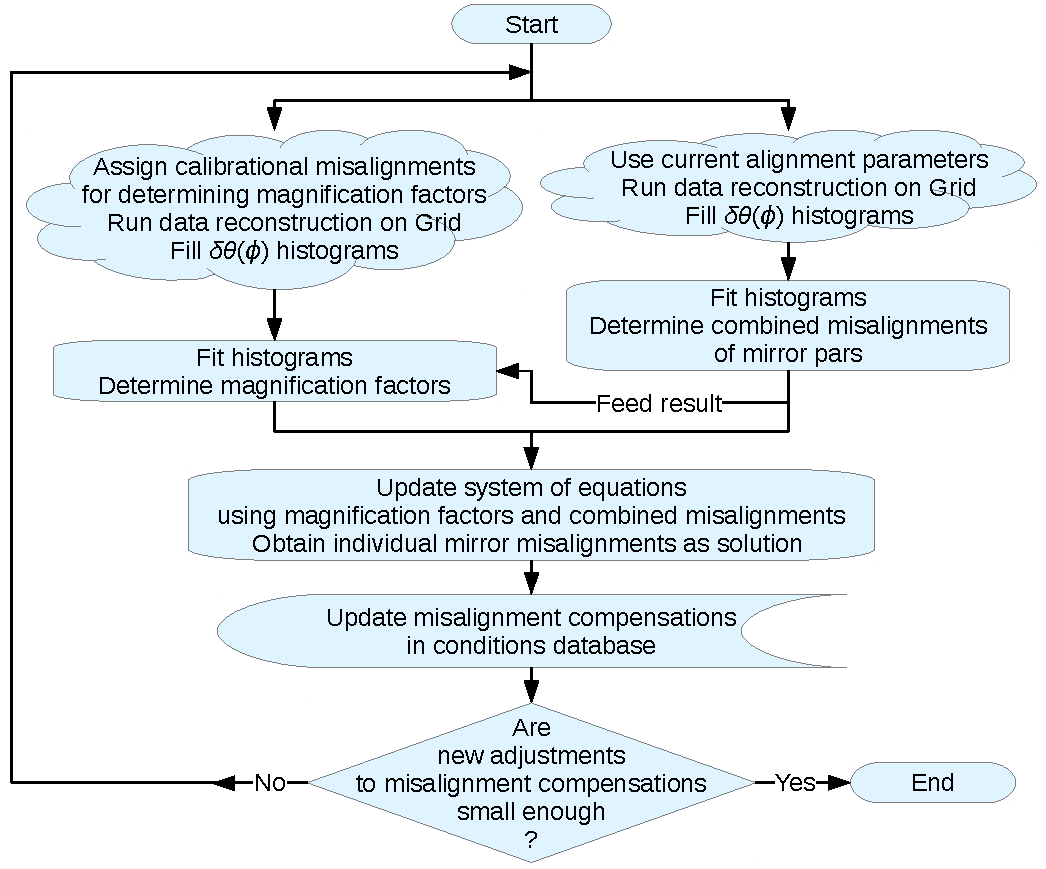
\includegraphics[width=1.0\textwidth]{figs/Framework/Workflow.pdf}
  \vspace{-1.0\baselineskip}
  \caption{
    Schematic diagram of the computing framework workflow steered by the \ganga
    script.}
  \label{fig:workflow}
  \vspace{-0.5\baselineskip}
\end{figure}

Currently, this software facility consists of a steering \ganga script, written
in Python, and three programs written in C++: a module that fills the
$\deltatheta(\phi)$ histograms necessary for determining possible mirror
misalignments while running the reconstruction over the preselected events
(see~\sect{sec:SelectionMethod}); a program that for every mirror combination
from the chosen subset finds combined tilts resulting from misalignments of both
primary and secondary mirror segments and a program that determines individual
misalignment compensating corrections for every mirror segment of both mirror
kinds.

This script runs a loop of iterations, each consisting of the following actions:
\begin{enumerate}
  \item
  run multiple data reconstruction jobs parallelized by \ganga across the Grid
  and produce $\delta\theta(\phi)$ histograms for every combination of one
  spherical and one flat mirror according to the optimized list of combinations
  determined in advance; this bunch of jobs forks into two groups, each running
  over the same set of DSTs but using different misalignment compensation
  values:
  \begin{enumerate}
    \item
    just up-to-date values
    \item
    additional calibrational tilts (e.g. $\pm 0.3\mrad$) are added to the
    up-to-date values of only one member of a combination at a time, for all
    combinations, in order to determine the magnification factors
    (see~\sect{subsec:Magnification})
  \end{enumerate}
  \item
  fit these histograms and determine for each combination its combined tilts
  around $y$- as well as $z$-axis in two case:
  \begin{enumerate}
    \item
    just as they are
    \item
    resulting from additional calibrational tilts
  \end{enumerate}
  \item
  magnification factors are calculated by dividing difference between biased
  combined tilts and the unbiased ones by the corresponding calibrational tilts
  \item
  update the system of linear equations using obtained magnification factors and
  total tilts; its solution is a set of individual tilts (around $y$ and $z$) of
  every segment
  \item
  update the existing misalignment compensations in CONDDB that were used during
  the current iteration
  \item
  if all the obtained adjustments to the previous misalignment corrections are
  (by absolute value) less than 0.1\unit{\mrad}, exit; otherwise continue.
\end{enumerate}
Because contents of CONDDB is stored in XML, we used Xerces-C++~\cite{Xerces311}
XML parser and XQilla~\cite{XQilla230} as an XQuery and XPath implementation to
alter the RICH mirror alignment adjustments in CONDDB.


%\section{Test on Monte Carlo}
\label{sec:MCTrial}

The alignment of the \lhcb RICH optical system was tested on simulated events.
The procedure described was applied to simulated events generated with a
misaligned optical system. \Fig{fig:RICHMCTest}
\begin{figure}[hbtp]
  \vspace*{-0.5\baselineskip}
  \centering
  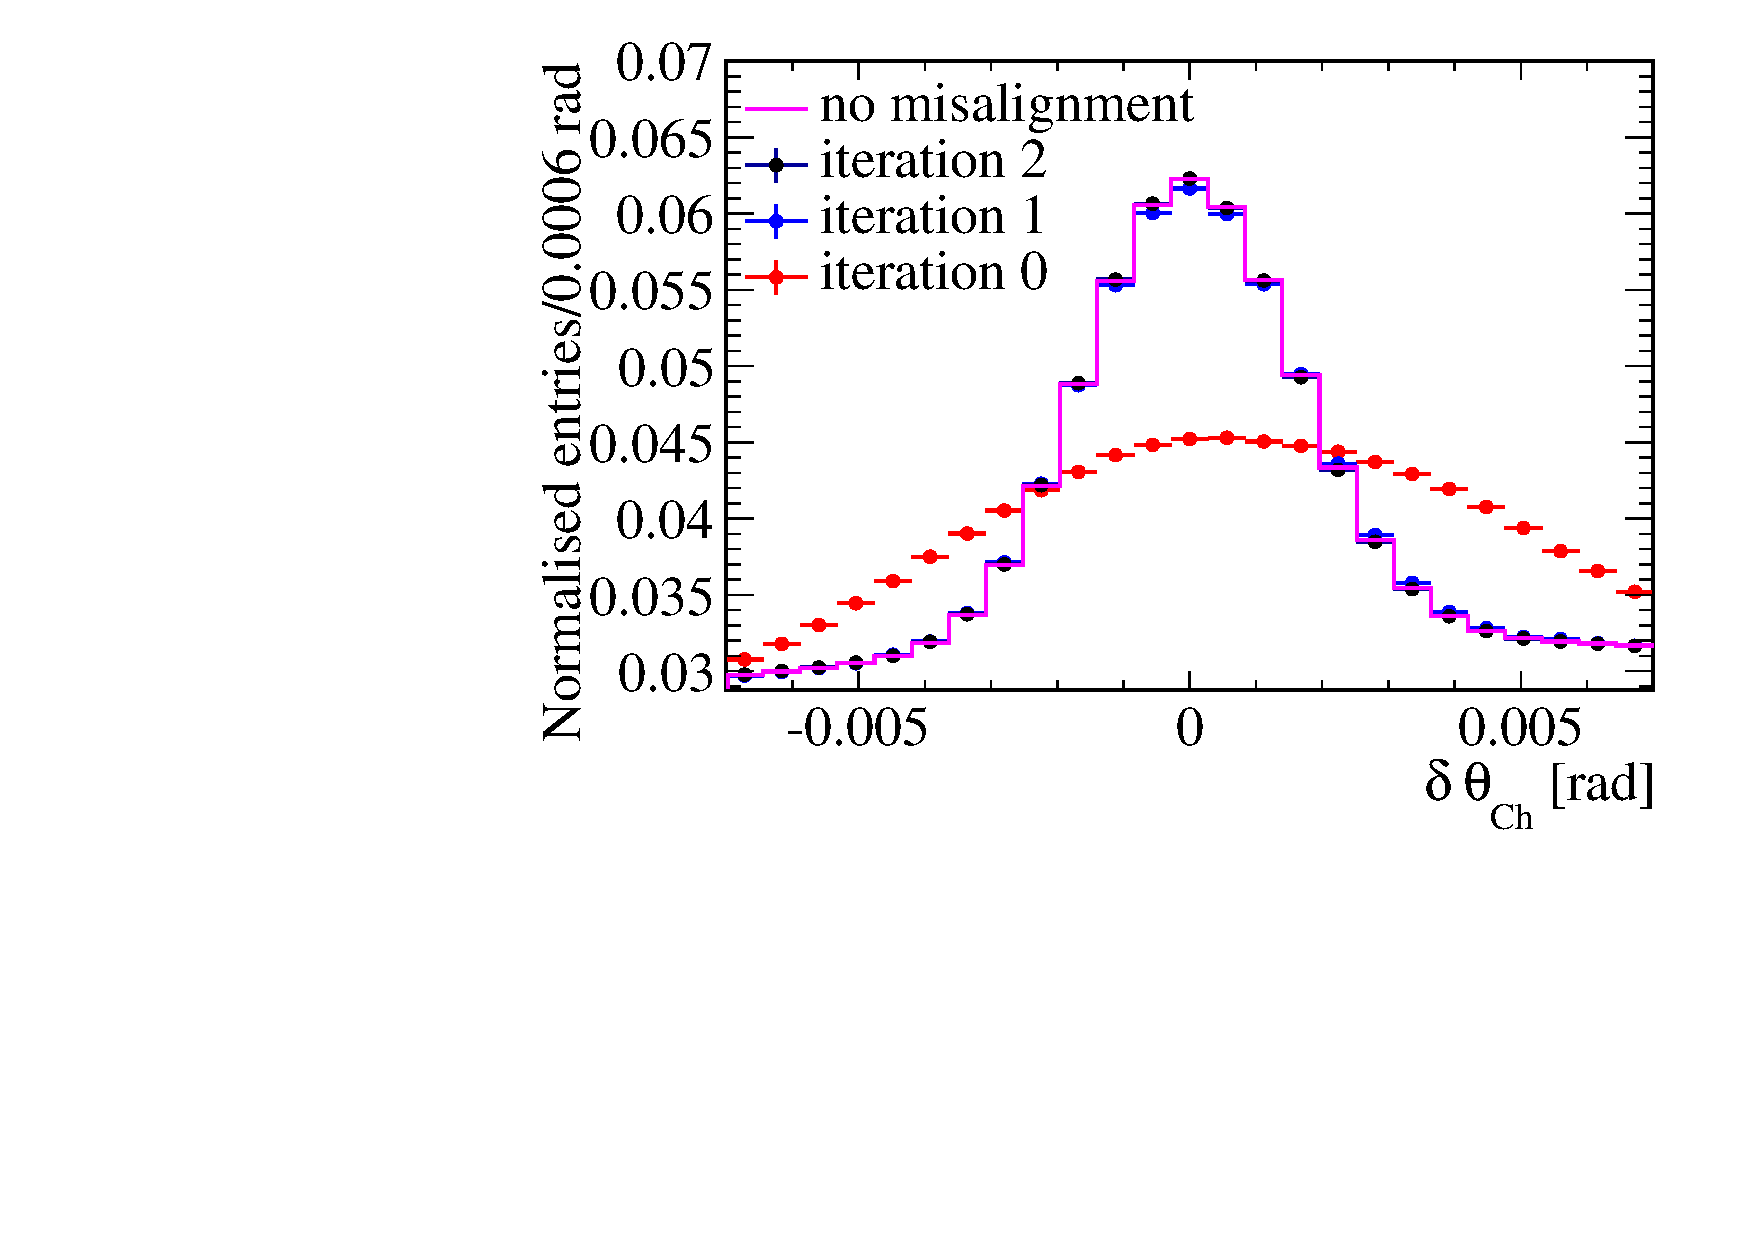
\includegraphics[width=0.49\textwidth, height=0.35\textwidth]
                  {figs/Results/RICH1_Alignment_MC10.pdf}
  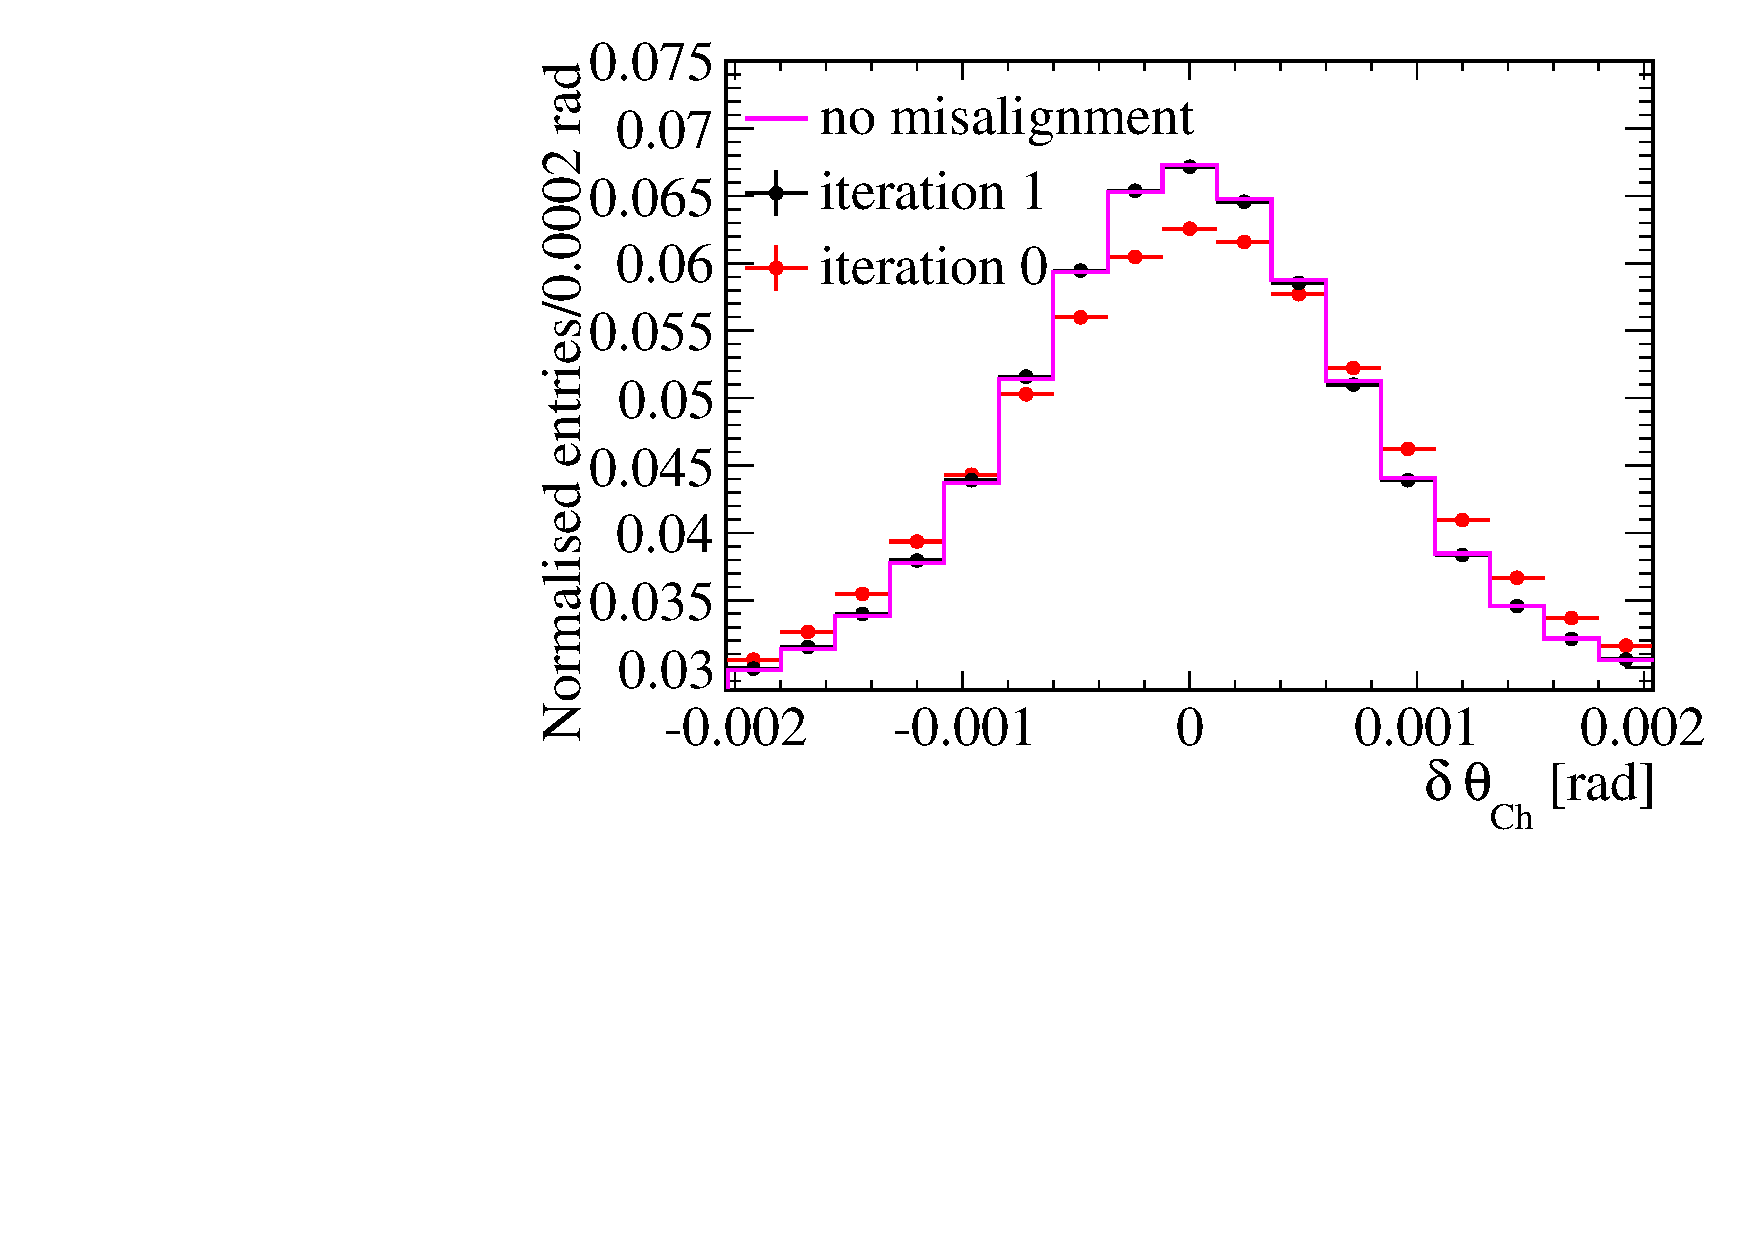
\includegraphics[width=0.49\textwidth, height=0.35\textwidth]
                  {figs/Results/RICH2_Alignment_MC10.pdf}
  \vspace*{-0.9\baselineskip}
  \caption{
    \deltatheta distribution for each iteration of the alignment procedure
    applied to misaligned Monte Carlo simulated data. Results are shown for the
    \richone detector (left) and the \richtwo  detector (right).}
  \label{fig:RICHMCTest}
  \vspace*{-0.5\baselineskip}
\end{figure}
shows the Cherenkov angle distribution for both RICH detectors after each
iteration of the alignment procedure, starting with the simulated misaligned
case. The results of this alignment are compared to those from simulated events
with a perfectly aligned system. Before convergence, each iteration of the
optical alignment procedure results in the distribution becoming closer to that
of the perfectly aligned case. The standard deviation of the \deltatheta
distribution for the RICH1 detector improves from $6.02\pm 0.04\mrad$ to
$1.563\pm 0.002\mrad$. Whereas for the \richtwo detector the resolution improves
from $0.772\pm 0.001\mrad$ in the misaligned case to  $0.668\pm 0.001\mrad$
after the alignment. The standard deviation for a perfectly aligned
\richone/\richtwo optical system is found to be  $1.569\pm
0.007\mrad$/$0.687\pm 0.003\mrad$.


\section{Alignment results}
\label{sec:AlignmentResults}

The alignment system presented here has been used throughout \lhcb data taking
since it began in 2010. The results shown here are from 2011 data applied to the
B\,hadron stream, using Stripping\,17 and Reco\,12. \deltatheta is plotted for
each iteration of the alignment process in~\fig{fig:RICHresolutionResults}.
\begin{figure}[hbtp]
  \vspace*{-0.5\baselineskip}
  \centering
  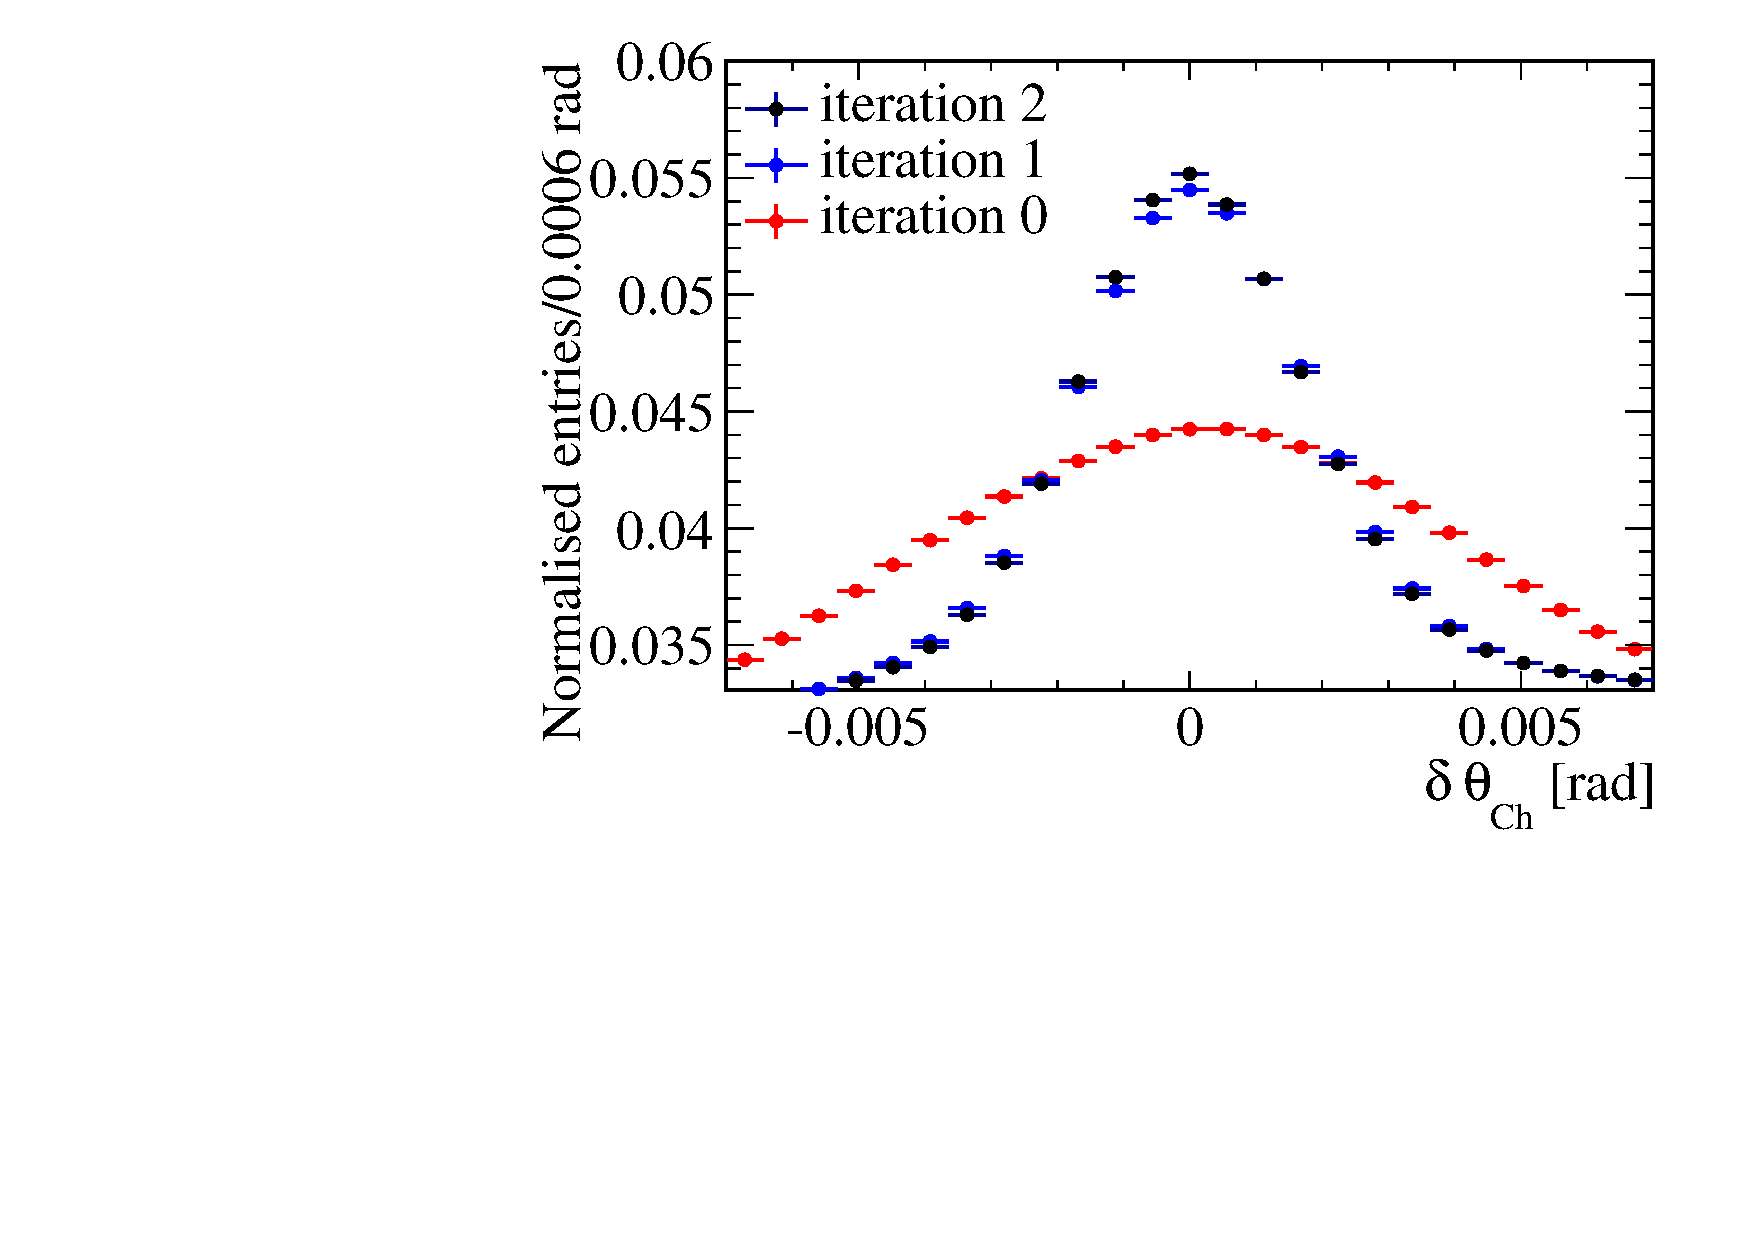
\includegraphics[width=0.49\textwidth]{figs/Results/RICH1_Alignment_2011.pdf}
  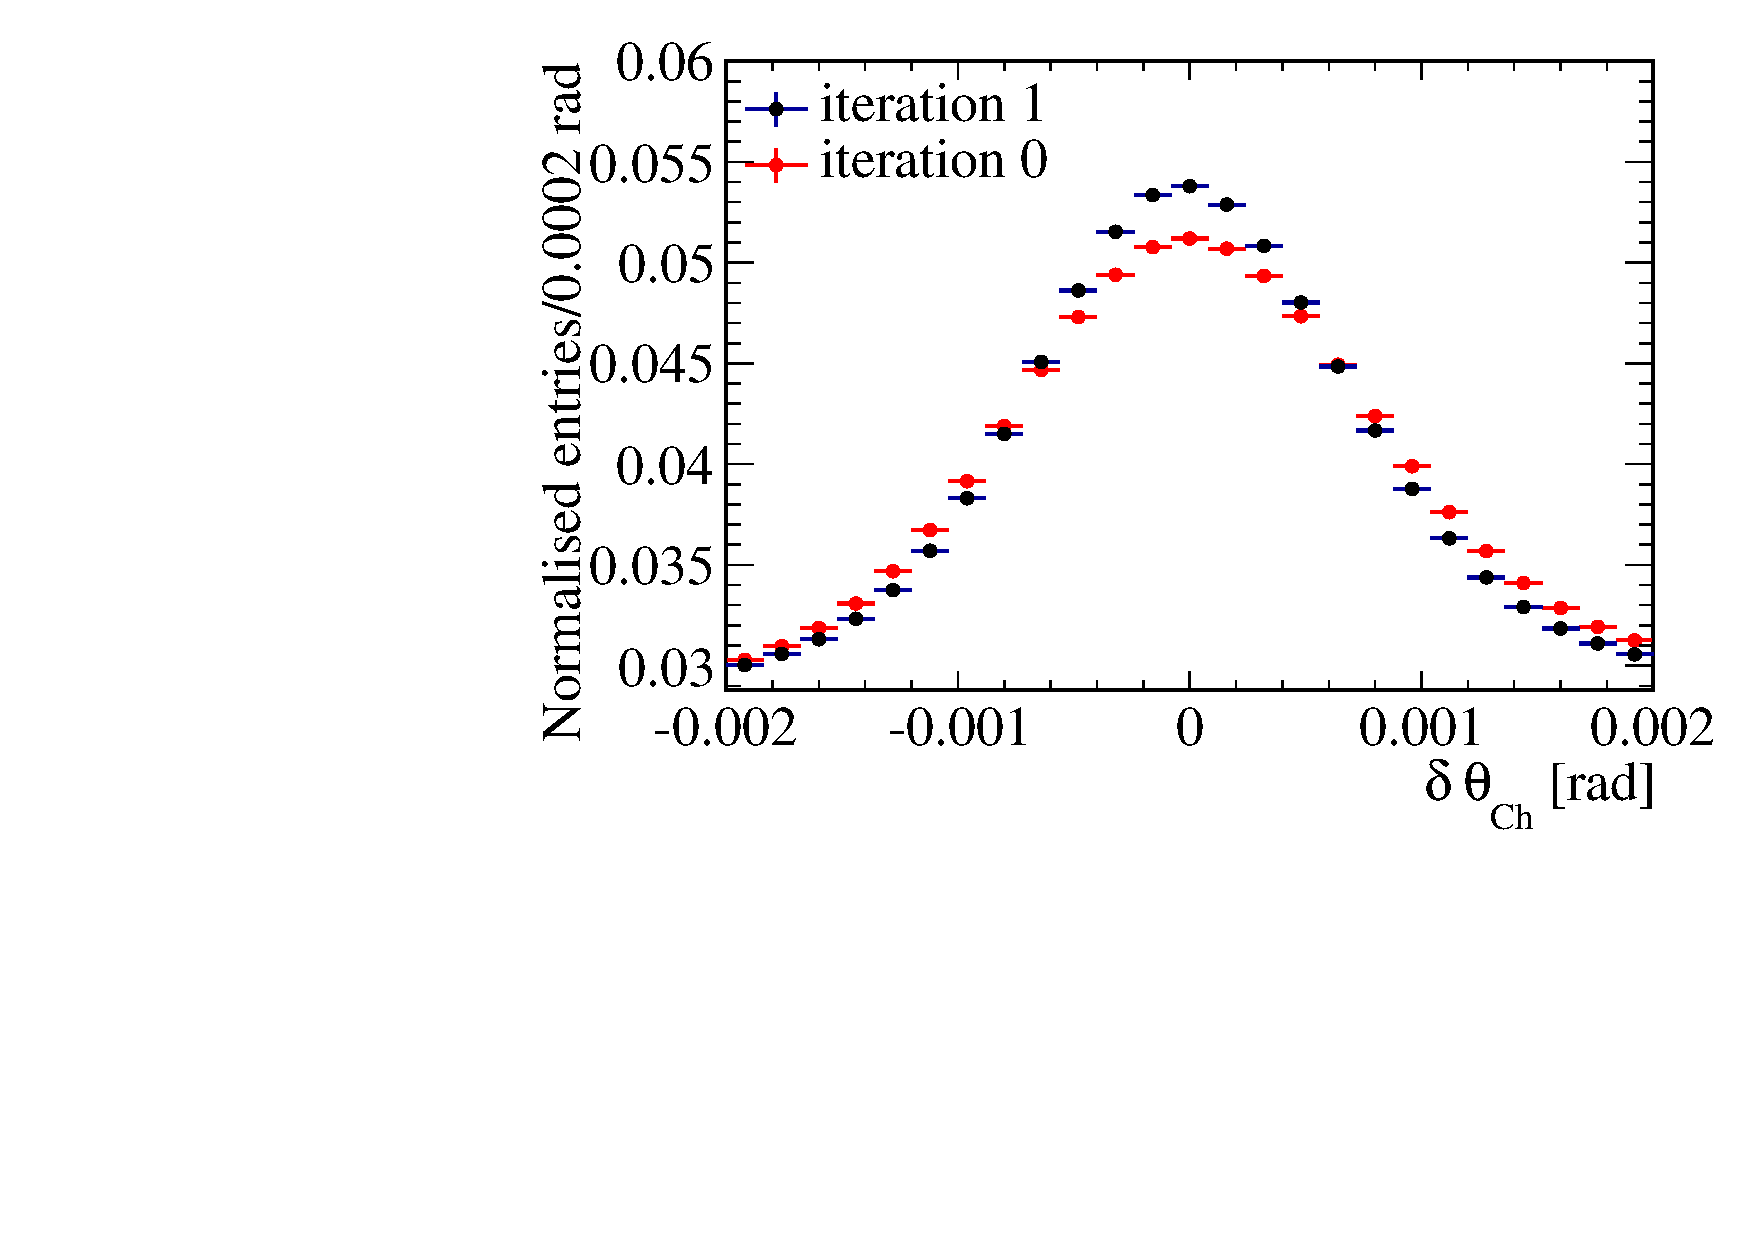
\includegraphics[width=0.49\textwidth]{figs/Results/RICH2_Alignment_2011.pdf}
  \vspace*{-0.9\baselineskip}
  \caption{
    \deltatheta is plotted for each iteration in the alignment of the \lhcb RICH
    optical system. \richone is shown on the left and \richtwo on the right. 
    Iteration 0 shows the \deltatheta distribution for the RICH detector with no
    software corrections for misalignments in the optical system. Corrections
    are then applied at each iteration until each mirror has a misalignment less
    than $0.1\mrad$ at which point the system is said to be aligned.}
  \label{fig:RICHresolutionResults}
  \vspace*{-0.5\baselineskip}
\end{figure}
Iteration~0 shows the resolution of the RICH detectors with no software
corrections for misalignments each subsequent iteration results in the
distribution getting closer to that of a perfectly aligned system.

Two iterations are required to align the mirrors of \richone from a state where
no corrections are assumed to an aligned state. Only a single pass is required
to align the optical system of the \richtwo detector. The extra iteration
required by the alignment procedure for \richone is believed to be due to the
initial conditions being much further than those for the aligned state.

The standard deviation of the \deltatheta distribution for \richone/\richtwo
without corrections (iteration 0) is $13.96\pm 0.05\mrad$/$0.73\pm
0.001\mrad$. This is improved to $1.602\pm 0.003\mrad$/$0.638\pm 0.0003\mrad$
after aligning the optical system of the RICH detectors, and compares to
$1.569\pm 0.007\mrad$/$0.687\pm 0.003\mrad$ for the perfectly aligned
\richone/\richtwo system.

The software alignment procedure for the \lhcb RICH mirrors has significantly
improved the resolution of both RICH detectors. However, the resolution  of the
\richone detector does not yet match that expected from simulation. There could
be many reasons for this including effects from the magnetic field.


\section{Conclusion} \label{sec:conclusions}

A method for alignment of the optical system of the \lhcb RICH detector
consisting of two sets of mirror segments installed in radiator vessels was
developed and presented. The developed method was tested with simulated events
and applied to data collected at the \lhcb experiment. The optical system is
aligned to within $0.1\mrad$, at which point the error due to mirror
misalignment becomes a small contribution.


\section{Acknowledgments} \label{sec:acknowledgments}

We are are grateful to Antonis Papanestis (RAL) for acquainting us with his
progress towards solving the problem of mirror alignment, to Chris Jones
(Cambridge) for photon reconstruction implementation, to all members of the
\lhcb RICH group and to Jonas Rademacker (University of Bristol) for numerous
discussions and consultations. Also we appreciate assistance of the \ganga team,
\lhcb core software group, Stefan Roisier (LCG group, CERN) and Lorenzo Moneta
(\root group, CERN).

 
% Do not include this in analysis note and conference reports
%\section*{Acknowledgements}

The text below are the acknowledgements as approved by the collaboration
board. Extending the acknowledgements to include individuals from outside the
collaboration who have contributed to the analysis should be approved by the
EB. The extra acknowledgements are normally placed before the standard 
acknowledgements, unless it matches better with the text of the standard 
acknowledgements to put them elsewhere.
They should be included in the draft of first circulation.
 
\noindent We express our gratitude to our colleagues in the CERN
accelerator departments for the excellent performance of the LHC. We
thank the technical and administrative staff at the LHCb
institutes. We acknowledge support from CERN and from the national
agencies: CAPES, CNPq, FAPERJ and FINEP (Brazil); NSFC (China);
CNRS/IN2P3 (France); BMBF, DFG, HGF and MPG (Germany); INFN (Italy); 
FOM and NWO (The Netherlands); MNiSW and NCN (Poland); MEN/IFA (Romania); 
MinES and FANO (Russia); MinECo (Spain); SNSF and SER (Switzerland); 
NASU (Ukraine); STFC (United Kingdom); NSF (USA).
The Tier1 computing centres are supported by IN2P3 (France), KIT and BMBF 
(Germany), INFN (Italy), NWO and SURF (The Netherlands), PIC (Spain), GridPP 
(United Kingdom).
We are indebted to the communities behind the multiple open 
source software packages on which we depend. We are also thankful for the 
computing resources and the access to software R\&D tools provided by Yandex LLC (Russia).
Individual groups or members have received support from 
EPLANET, Marie Sk\l{}odowska-Curie Actions and ERC (European Union), 
Conseil g\'{e}n\'{e}ral de Haute-Savoie, Labex ENIGMASS and OCEVU, 
R\'{e}gion Auvergne (France), RFBR (Russia), XuntaGal and GENCAT (Spain), Royal Society and Royal
Commission for the Exhibition of 1851 (United Kingdom).

 
%\input{appendix}
 
% This should be taken out in the final paper
%\input{supplementary-app}
 
\addcontentsline{toc}{section}{References}
\setboolean{inbibliography}{true}
\bibliographystyle{LHCb}
%\bibliographystyle{plain}
\bibliography{SoftwareMirrorAlignment}
 
\end{document}
